\appendix
\section{Application Scenarios of Query Privacy}
\label{app:query-privacy-app}

Due to legal regulations (\eg GDPR~\cite{GDPR}), protecting \textit{data privacy} is now common in real-life scenarios, especially when spatial location implies the travel patterns or trajectories of a user. 
\textit{Query privacy} is equally important has numerous application scenarios. Here are some detailed examples:

\begin{enumerate}
    \item \textbf{Navigation}: Apps like Google Maps \cite{googlemaps} and Waze \cite{waze} frequently query user locations to provide directions and traffic updates. Revealing exact locations can expose sensitive information about users' daily routines and personal lives.
    
    \item \textbf{Social Networking}: Platforms like Facebook \cite{facebook} and Instagram \cite{instagram} allow users to check in at various locations. Protecting the privacy of these check-ins is crucial to prevent stalking and harassment.
    
    \item \textbf{Location-based Advertising}: This service targets users based on their current or recent locations. Protecting user privacy ensures that advertisers do not have access to sensitive location data, which could be misused for targeted marketing.

    \item \textbf{POI Search}: Applications like Yelp \cite{yelp} and TripAdvisor \cite{tripadvisor} allow users to search for nearby points of interest like restaurants, cafes, or hotels. Ensuring the privacy of sensitive location data will prevent potential tracking and profiling of users’ movement patterns by the platform.
\end{enumerate} 

Please refer to \cite{DBLP:reference/sp/2018mdp,DBLP:conf/esorics/2009-5599} for more application scenarios of query privacy.

\section{Security Analysis}
\label{app:secure}
The security analysis of our query rewriter is based on the composition lemma in \cite{goldreich2009foundations} (see its Sec. 7.3.1).
The lemma states that given a secure protocol $\pi^{g|f}$ that can securely compute $g$ based on a plaintext query $f$ and a secure protocol $\pi^f$ for operation $f$, the operation $g$ can be securely computed by executing protocol $\pi^{g|f}$ but substitutes every plaintext query $f$ with an execution of $\pi^f$.

We prove the security of query rewriter for asymmetric federated queries (\appref{app:secure-asym}) and symmetric federated queries (\appref{app:secure-symm}) separately.
Finally, we present a case study on attacking asymmetric federated range counting in \appref{app:secure-case}.

\subsection{Security Analysis of Asymmetric Federated Queries}\label{app:secure-asym}

In the following, we conduct a thorough analysis of the security of asymmetric federated queries in \sysname, categorizing them into two distinct kinds: \textit{radius-known queries} and \textit{radius-unknown queries}. 

\begin{itemize}
    \item \textbf{Security of Radius-Known Queries.} Federated range query, range counting and distance join belong to \textit{radius-known queries}.
    For \textit{federated range query} and \textit{distance join}, the secure protocol $\pi^{g|f}$ is the secure set union (\defref{def:ssun}) based on the query results of one or multiple plaintext range queries over the federation.
    The protocol $\pi^f$ corresponds to the plaintext range query (\defref{def:prq}).
    The protocol $\pi^f$ is secure, since the plaintext range query only occurs in each silo, which will not leak any information to other silos.
    From the composition lemma, federated range query and distance join are secure against semi-honest adversaries.
    Federated range counting is also secure based on a similar proof (\ie replacing $\pi^{g|f}$ with the secure summation in \defref{def:ssum} and $\pi^f$ with the plaintext range counting in \defref{def:prq}).
    
    \item \textbf{Security of Radius-Unknown Queries.} The federated kNN query and kNN join belong to \textit{radius-unknown queries}.
    For federated kNN query (\algref{alg:knn}), let protocol $\pi^f$ be the secure count comparison between $k$ and the local counts.
    The security of $\pi^f$ can be proved in the same way as before.
    Denote protocol $\pi^{g|f}$ as \algref{alg:knn} based on the plaintext count comparison query.
    We then show protocol $\pi^{g|f}$ is also secure.
    Assuming semi-honest adversaries, each silo can simulate its view of the execution of the protocol.
    Specifically, knowing the range $[l, u]$ used at the beginning of a round, each silo can compute $\thres$ used in that round.
    If $\thres$ is the same as the final radius, it concludes that the protocol must have ended in this round.
    Otherwise, it simply updates the range to that side of $\thres$ which contains the final radius.
    Along with the knowledge of the initial range, this shows that each silo can simulate the execution of the protocol, which means the protocol $\pi^{g|f}$ is secure.
    Thus, our \algref{alg:knn} is secure against semi-honest adversaries based on the composition lemma.
    The security of federated kNN join can be proved similarly.
\end{itemize}

\subsection{Security Analysis of Symmetric Federated Queries}\label{app:secure-symm}

Similar to the previous security analysis, we analyze the security of symmetric federated queries in \sysname from two categories: \textit{radius-known queries} and \textit{radius-unknown queries}. 

\begin{itemize}
    \item \textbf{Security of Radius-Known Queries.} 
    For \textit{federated range query}, the secure protocol $\pi^{g|f}$ employs the secure distance comparison (\defref{def:sdcmp}), which relies on the fully homomorphic encryption (FHE) scheme (\ie the BGV scheme \cite{DBLP:journals/csur/AcarAUC18}), and the secure set union (\defref{def:ssun}).
    The protocol $\pi^f$ corresponds to the plaintext range query (\defref{def:prq}).
    It is secure because the plaintext range query is executed within each silo individually, thereby preventing any information leakage to other silos.
    According to the composition lemma, the query rewriter for symmetric federated range queries ensures data privacy.
    Regarding the additional privacy requirement of query privacy, the secure protocol, secure location perturbation (\defref{def:sdp}), is based on the BPL mechanism in \cite{DBLP:journals/corr/abs-2312-12012}.
    This mechanism has been proven to satisfy $(\epsilon,\delta)$-Geo-Indistinguishability (Geo-I) \cite{DBLP:conf/ccs/AndresBCP13}, a widely-adopted privacy notion for preserving location privacy.
    Thus, the query privacy is due to the protection of query location with secure location perturbation.
    As for \textit{federated distance join}, the data privacy and query privacy can be guaranteed, since a federated distance join is decomposed into a series of federated range queries, and the security of each federated range query has been proven.
    The security of \textit{federated range counting} shares similarities with that of federated range query, primarily due to their near-identical decomposition plans (see \tabref{tab:sym-rewriter}).
    However, a key difference lies in the nature of their query answers. 
    While federated range query requires a secure set union to collect spatial objects falling within the specified range, federated range counting simply returns an integer count as its output. 
    This distinction underscores the minimal exposure of information in federated range counting, further reinforcing its security.
    
    \item \textbf{Security of Radius-Unknown Queries.} 
    To prove the security of radius-unknown queries, we only need to show the security of federated kNN query,
    since a federated kNN join is decomposed into multiple independent federated kNN queries by \sysname.
    Similar to the decomposition plan for asymmetric federated kNN query, the query rewriter for symmetric federated kNN query also utilizes a binary-search procedure.
    The key difference is that the initial upper bound is determined by plaintext kNN queries and secure location perturbation.
    Thus, for this step, the secure protocol $\pi^{g|f}$ is due to the privacy guarantee of $(\epsilon,\delta)$-Geo-Indistinguishability (Geo-I) \cite{DBLP:conf/ccs/AndresBCP13}.
    The security analysis for the other steps is similar to that for asymmetric radius-unknown queries.
\end{itemize}

\subsection{Case Study on Semi-Honest Attack}\label{app:secure-case}

\begin{table}[t]
    \centering
    \caption{A case study on hacking (asymmetric) federated range counting in \sysname.}
    \begin{small}
    \begin{tabular}{ccc}
		\toprule
		\makecell[c]{Colluded\\silos} & \makecell[c]{Attack\\success rate}  & \makecell[c]{Running\\time}  \\
		\midrule
		1             & $0$         & No result for 2 months    \\
		2             & $0$         & No result for 2 months    \\
		3             & $0$         & No result for 2 months    \\
% 		4             & $2.56\%$    & 173.23 s       \\
		\bottomrule
    \end{tabular}
    \end{small}
    \label{tab:attack}
\end{table}

\fakeparagraph{Case Study}
We have also conducted a case study to show how \sysname defenses against the semi-honest adversaries when processing asymmetric federated range counting.

\begin{itemize}
    \item \textbf{Experimental Setup.} The case study is based on the BJ dataset with 6 silos (\ie our default setting) and we vary the number $m$  of colluded adversaries (\ie silos) from 1 to 3. Then, when processing asymmetric federated range counting, the attack will occur at the only secure operator (\ie secure summation \cite{DBLP:journals/dke/EmekciSAA07}). To attack the secure summation, we use the method introduced in ~\cite{DBLP:journals/dke/EmekciSAA07}. In general, a secure operator successfully defenses against the attack, if adversaries cannot get any feasible result after a long time (\eg two months in our experiment). Furthermore, the other experiment parameters are the same as those in \secref{subsec:exp-cmp}.
    
    \item \textbf{Experimental Result.} 
    As shown in \tabref{tab:attack}, even when 50\% of the silos collude, they cannot infer any feasible result even after two months' cracking.
    Note that it is commonly assumed in existing work that the portion of colluded adversaries is less than 50\%.
    Based on the computational security \cite{DBLP:reference/dbsec/2008,goldreich2009foundations,DBLP:conf/ccs/Bayatbabolghani18}, this result proves \sysname is hard to attack.
\end{itemize}

\section{Handling Ties in Symmetric Federated kNN Query}
\label{app:knn-tie}

We provide a solution for handling ties in symmetric federated kNN query and conduct an experimental comparison.
\textbf{Main Idea.} To break our assumption and handle the special case of ties, we need to address two question: (1) how to identify such cases and (2) how to retrieve exactly $k$ nearest neighbors, using the following ideas:
\begin{enumerate}[(1)]
    \item \textbf{Identify such cases}.
    For any searching radius $r$ during the binary-search, whenever the total number of spatial objects closer to the query object $q$ than $r$ is equal to $k$ (\ie the result of secure count comparison is $sign = 0$), we can find exactly $k$ nearest neighbors (\ie there are no other objects whose distances to $q$ are also the $k$th nearest distances).
    When the binary-search terminates and $sign$ is always non-zero, we will encounter the mentioned case (we call it ``ties'' for brevity).
    
    \item \textbf{Retrieve exactly $k$ nearest neighbors}.
    Under this case, we will obtain the final lower bound $l$ and upper bound $u$ of the searching radius for $k$th nearest neighbor.
    Since the binary-search has been terminated, we can derive that $u-l$ must be smaller than the distance precision $\epsilon_0$.
    Now, we \textit{first} use the circular range $\text{circle}(q,l)$ to locate all spatial objects that are strictly inside the circle curve (\ie by a symmetric federated range query), and denote the total count as $k_l$.
    Notice that we can temporarily cache the partial answers in each data silo at this step.
    \textit{Next}, we only need to randomly pick $k-k_l$ spatial objects from those objects on the circle curves.
    To achieve this goal, we sequentially request such spatial objects from every data silo,
    and set a limitation on how many spatial objects are indeed required.
    \textit{Lastly}, a secure set union operator is used to collect the $k$ nearest neighbors, since the partial answer has been cached in each data silo.
\end{enumerate}

\begin{figure}[t]
    \centering
    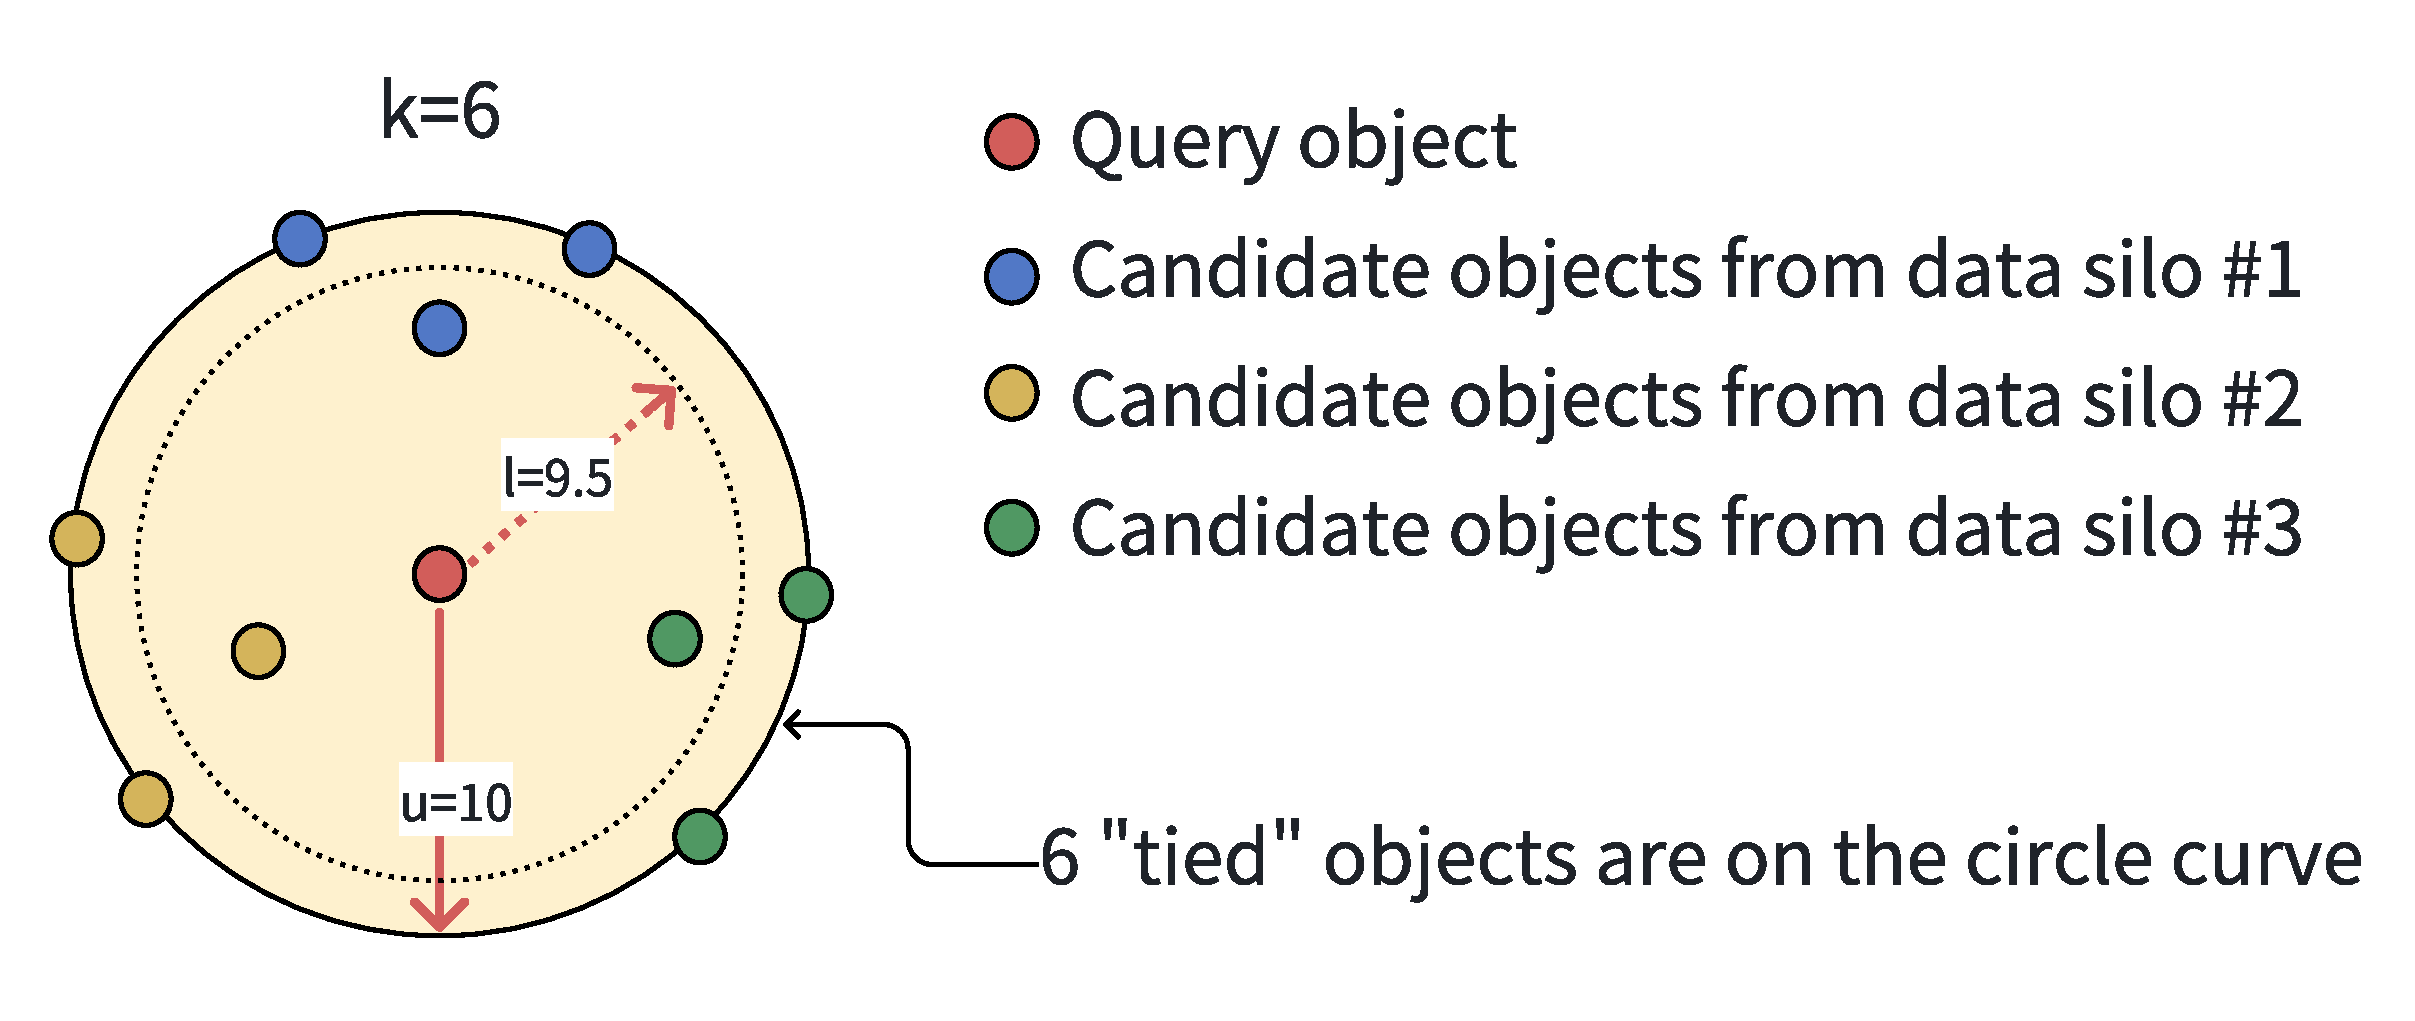
\includegraphics[width=0.45\textwidth]{apdx/example.pdf}
    \caption{Illustration of the special case of symmetric federated kNN query ($k=6$).}
    \label{fig:special-knn}
\end{figure}

\algref{alg:tie-knn} illustrates the detailed procedure of using the main idea to process the cases of ties.
Specifically, lines 3-9 represent the procedure of binary-search.
In line 10, when $sign$ equals 0 in some iteration of the binary search, we know the current searching radius $\thres$ is already enough to retrieve the exact $k$ nearest neighbors.
A symmetric federated range query can drive the query answer.
By contrast, in line 12, $sign$ has never become $0$, then we know we are facing the case of ties now.
To handle this case, line 14 computes how many data objects are strictly inside the circle curve, denoted by $k_l$.
Thus, we only need to pick $k-k_l$ from those tied objects on the circle curve.
To do so, lines 16-20 sequentially request certain objects from each data silo, and limit the number of retrieved object no larger than $remain$ (since we do not need more).
To avoid data objects are duplicate statistics, lines 14 and 17 will cache the (partial) answer locally at each silo.
Finally, line 20 collects the query answer from all data silos.

To ease of understanding, \expref{exp:special-knn} is used to further illustrate the main idea.

\begin{example}\label{exp:special-knn}
    \figref{fig:special-knn} illustrates an instance as you mentioned,
    where $k$ is 6 and the distance precision $\epsilon_0$ is set to 1.
    \Song{Suppose the final upper bound $u$ is 10, and the final lower bound $l$ is 9.5.}
    When using the upper bound $u$ of 10 as the radius, the number of points is 9, which exceeds $k$. 
    When using the lower bound $l$ of 9.5 as the radius, the number of points is 3, which is fewer than $k$. 
    Since the difference between the bounds, $u-l=0.5$, is less than the distance precision $\epsilon_0=1$, the binary search has been terminated and we can identify the case of ties.
    As shown in \figref{fig:special-knn}, this case introduces a challenge in handling boundary points to ensure that exactly $k$ spatial objects are retrieved as the $k$ nearest neighbors. 
   To address this issue, we use the following strategy to manage these boundary spatial objects. 
   
   \begin{enumerate}[(1)]
    \item
    % during the binary-search process, each silo caches the sets of all points corresponding to both the upper and lower bounds.
    We perform a symmetric federated range query with the query object $q$ (marked in red color in \figref{fig:special-knn}) and the circle radius $l = 9.5$.
    The query answer (\ie the three objects within the inner circle) will be cached individually within each data silo.
    Besides, these data silos collaboratively and securely compute the total count $k_l = 3$.
    
    % In this example, when querying with the upper bound, each silo caches 3 points, resulting in a total of 9 points, with the cache for each silo denoted as $Cand_i$. When querying with the lower bound, each silo caches 1 point, totaling 3 points, with the cache for each silo denoted as $Cand_i’$.
    
    \item Now, it is still 3 objects short of the required $k = 6$ objects.
    Moreover, we do not know the exact number of ties in each data silo, but need to retrieve exactly 3 additional objects from tied ones.
    Thus, we need to sequentially request up to 3 points from each silo. 
    Specifically, starting from data silo \#1, we perform a symmetric federated range query with the query object $q$ and the circle radius $u = 10$ in data silo \#1, and limit the number of (uncached) query answer to 3.
    Although there are three objects within the query area, one of them has already been cached before, meaning data silo \#1 can only provide two more answers as the $k$ nearest neighbors.
    After this step, we need to request one more point from data silos \#2 and \#3.
    Similarly, we perform a symmetric federated range query with the query object $q$ and the circle radius $u = 10$ in data silo \#2, and limit the number of (uncached) query answer as 1.
    In data silo \#2, three objects are within the query range, but one has been cached. 
    Then, data silo \#2 can randomly pick one from the two uncached points as the cached query answer. 
    At this point, we have obtained exactly $6$ spatial objects as the query answer, thus eliminating the need to request any additional (uncached) objects from data silo \#3.
    
    \item \textit{Lastly}, a secure set union is performed to collect all the cached spatial objects from the data silos, resulting in a final output that contains exactly the 6 nearest neighbors.
    \end{enumerate}
\end{example}


\setlength{\textfloatsep}{1ex}
\setlength{\floatsep}{1ex}
\begin{algorithm}[t]
	\caption{\small{Symmetric federated kNN query}}\label{alg:tie-knn}
	\KwIn{federation $F$, query object $q$, integer $k$}
	\KwOut{the (exact) query answer $ans$}
    $[l,u] \gets [0,U]$, where $U$ is the tight upper bound\;
    $q' \gets$ secure location perturbation $\geoi(q)$\;
    \While {$u - l \geq \epsilon_0$} {
        $\thres \leftarrow (l+u)/2$, $\mathcal{R} \gets \text{circle}(q, \thres)$\;
        $v_i \gets$ symmetric federated range counting in $F$ with circular range $\mathcal{R}$\; 
        $sign \gets$ secure count comparison $\scmp(\{v_i\}, k)$\;
        \textbf{if} $sign < 0$ \textbf{then} $l \leftarrow \thres$\;
        \textbf{else if} $sign > 0$ \textbf{then} $u \leftarrow \thres$\;
        \textbf{else} \textbf{break}\;
    }
    \If{$sign=0$}{
        % \ForEach(// perform in parallel){silo $F_i \in F$}{
        $ans \gets$ symmetric federated range query in $F$ with circular range $\text{circle}(q, \thres)$\; 
        % $ans$ $\gets$ secure set union $\ssun(S_1,\cdots,S_n)$\;
        % } 
        % $S_i \gets$ plaintext range query $\lrq(F_i, circle(q, \thres))$\;
    }
    \Else(// identify cases of ties \& retrieve exact kNN){
        $\mathcal{R}_l \gets \text{circle}(q, l)$,
        $\mathcal{R}_r \gets \text{circle}(q, r)$\;
        $k_{l} \gets$ symmetric federated range counting in $F$ with circular range $\mathcal{R}_l$ and cache all the spatial objects that are inside $\mathcal{R}_l$ locally at each silo\;
        \tcp{need to retrieve exactly $remain$ objects}
        $remain \gets k - k_{l}$\; 
        \ForEach(// perform in sequential){silo $F_i \in F$}{ 
            $k_r^i \gets$ symmetric federated range counting in $F_i$ with circular range $\mathcal{R}_r$ over uncached spatial objects at silo $F_i$, limit the query answer to $\le remain$, and cache the query answer locally at silo $F_i$\;
            $remain \gets remain - k_r^i$\;
            \lIf{$remain=0$}{\textbf{break}}
        }
        $ans$ $\gets$ secure set union $\ssun(S_1,\cdots,S_n)$ over all cached spatial objects within each data silo\;
    }
    \KwRet{$ans$}\;
\end{algorithm}
\afterpage{\global\setlength{\textfloatsep}{\oldtextfloatsep}}
\afterpage{\global\setlength{\floatsep}{\oldfloatsep}}

\textbf{Experimental Setup.}
Since we have not found such cases in our datasets (OSM and BJ), we generate a new synthetic dataset to conduct this experiment.
In the new synthetic dataset, there are six data silos and each data silo has 10,000 spatial objects.
We also fix $k$ as 16 (\ie our default setting) and vary the proportion (denoted by $\alpha$) of spatial objects strictly inside circle curve 25\%, 50\%, 75\%, and 100\%, respectively.
We also ensure that at least 16 spatial objects happen to be on the circle curve (\ie they are ``ties'').
In other words, when $\alpha=25\%$, $(1-25\%) \cdot k = 12$ spatial objects in the query answer are on the circle curve.
Similarly, when $\alpha=100\%$, no spatial object in the query answer is on the circle curve.

\begin{figure}[t]
    \centering
    \begin{subfigure}{0.48\textwidth}
        \centering
        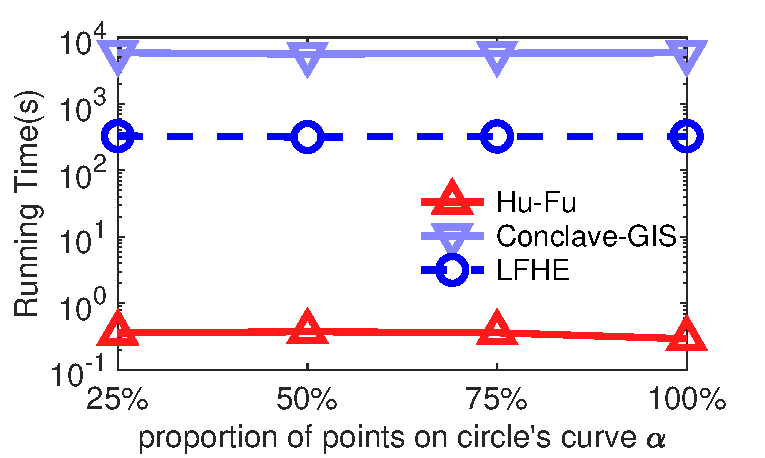
\includegraphics[width=0.48\linewidth]{apdx/random_knn_corner_time.pdf}
        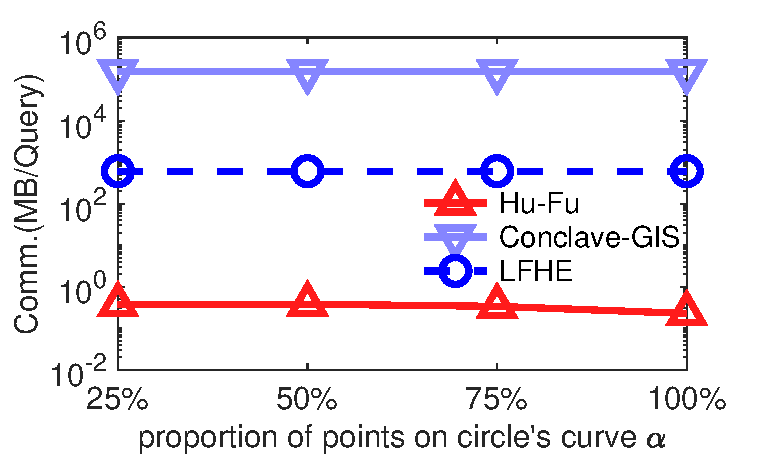
\includegraphics[width=0.48\linewidth]{apdx/random_knn_corner_comm.pdf}
    \end{subfigure}
    \caption{Performance of \Song{symmetric} federated kNN query in the synthetic dataset for handling ties.}
    \label{fig:random-knn-corner}
\end{figure}

\textbf{Experimental Result.}
\figref{fig:random-knn-corner} shows the experimental result. 
We can observe that our solution \sysname is still more efficient than the other baselines.
%The algorithm’s performance is not significantly affected by the proportion of spatial objects within the circle and remains relatively stable overall. 
Additionally, we also evaluate the total cost of our solution to the above two technical issues (\ie identifying the case of ties and retrieving exactly $k$ nearest neighbors).
The total time cost of these two steps remains within 400ms, and the communication cost stays under 400KB, accounting for 4.4\% of the total query time and 0.17\% of the total communication cost.

\section{Additional Experiments on Heterogeneous Data Silos}\label{app:exp-2}

\begin{figure}[t]
    \centering
    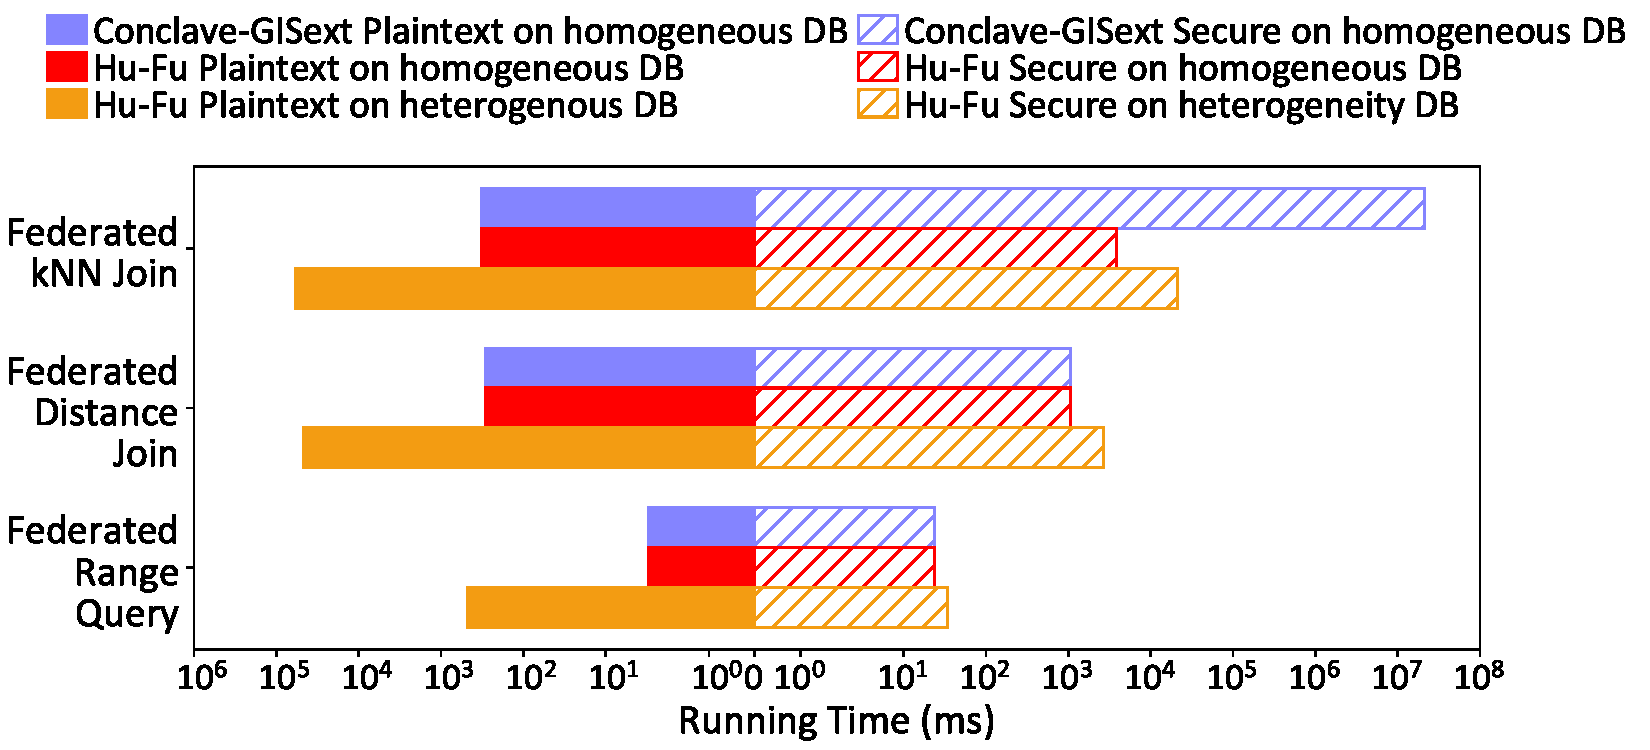
\includegraphics[width=0.48\textwidth]{apdx/database_compare_range.pdf}
    \caption{Running time breakdown.}
    \label{fig:database-cmp-range}
\end{figure}

\figref{fig:database-cmp-range} shows the results of asymmetric federated range query, distance join, and kNN join in the experiment of heterogeneous silos.
We can first observe that our \sysname can support all six spatial database systems, including PostGIS~\cite{postgis}, MySQL~\cite{mysql}, SpatiaLite~\cite{spatialite}, Simba~\cite{sigmod16simba}, GeoMesa~\cite{ds15geomesa}, and SpatialHadoop~\cite{icde15spatialhadoop}.
In addition, for all federated spatial queries in \figref{fig:database-cmp-range}, we observe the running time of \sysname becomes longer, compared with the results of homogeneous silos (\ie PostGIS in this test).
This is because the time cost of \sysname's plaintext primitives (\ie plaintext range query) increases due to the slowest spatial database system.
We can also observe that the experimental patterns of federated distance join and federated kNN join are similar to those of federated range query and federated kNN query.
This is because a federated distance/kNN join is decomposed into a series of federated range/kNN query.
Besides, we also recommend that all silos can use more efficient spatial database systems to further speed up the federated spatial queries.

This observation also holds for processing symmetric federated spatial queries, since the query processing procedure also involves plaintext primitives such as the plaintext range query and kNN query.

\begin{figure}[t]
    \centering
    \begin{subfigure}{0.45\textwidth}
        \centering
        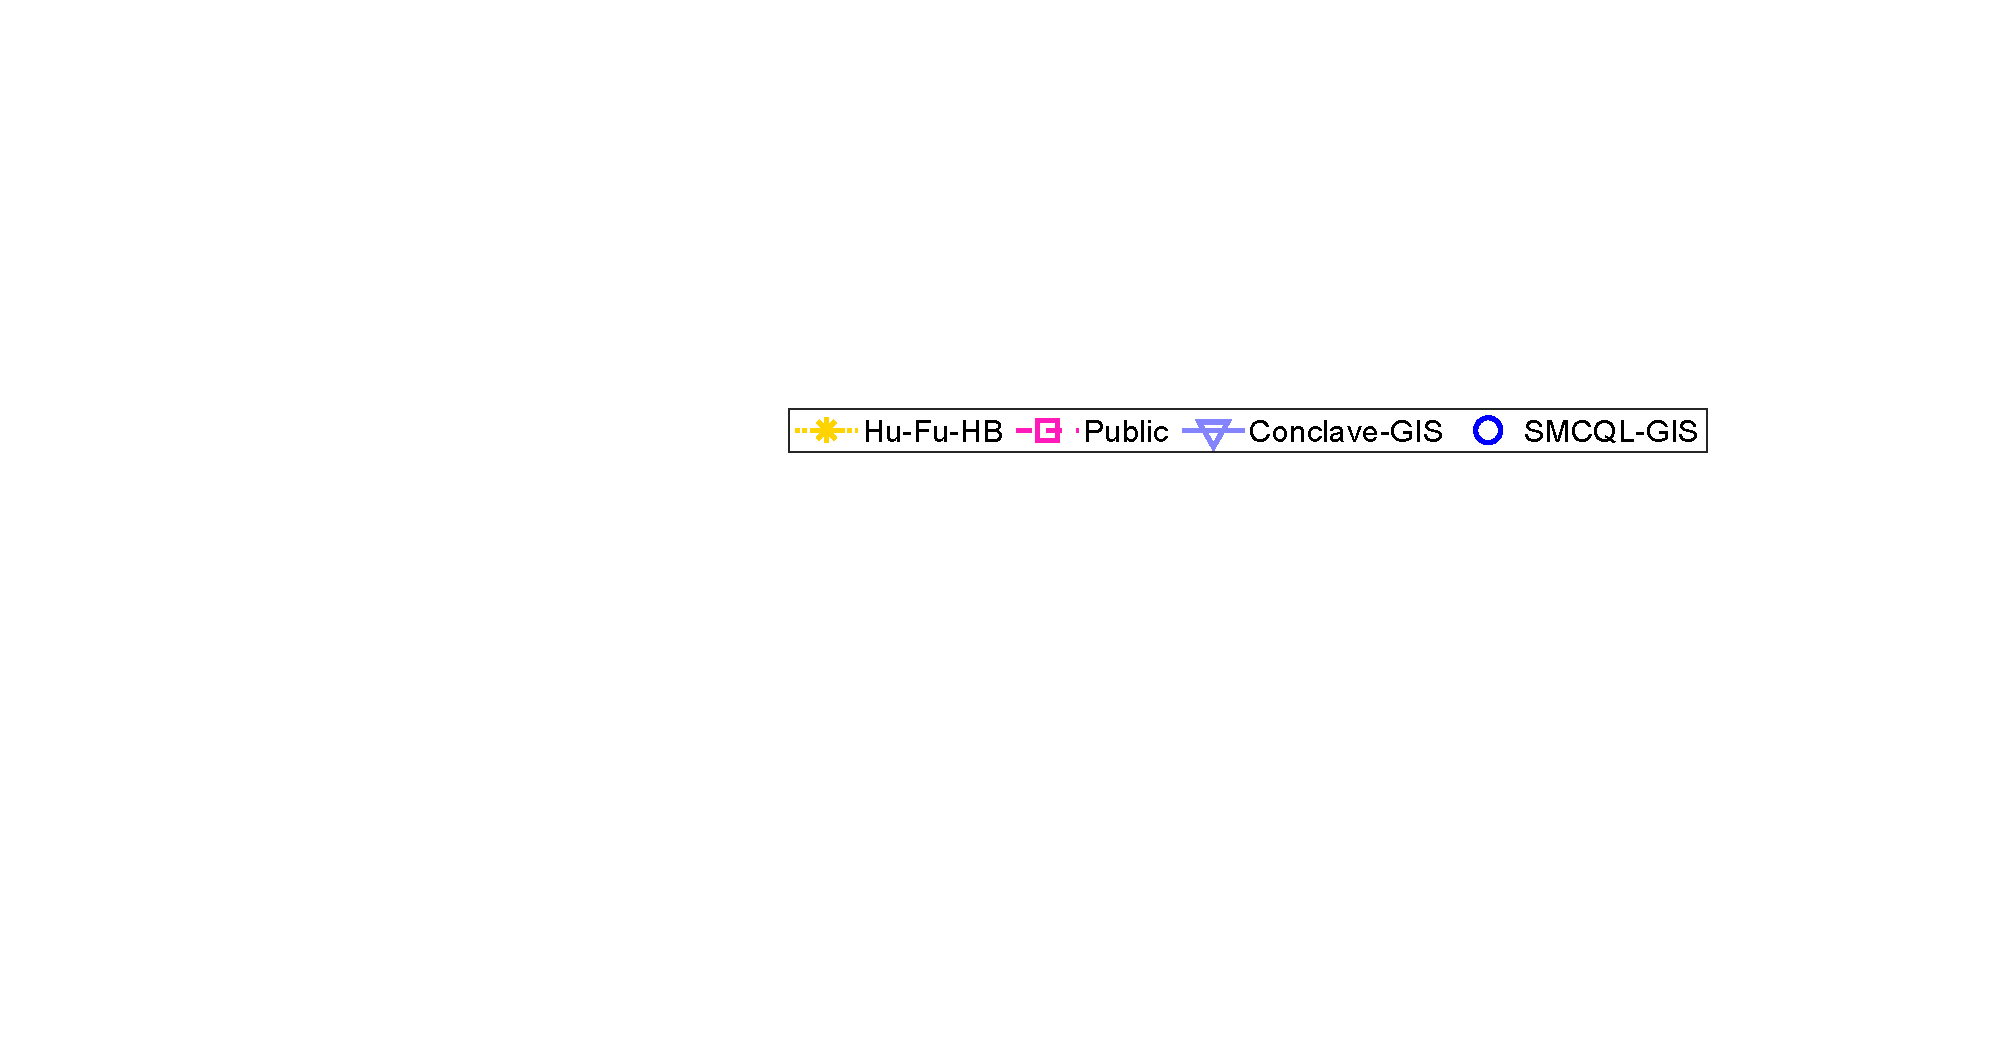
\includegraphics[width=\textwidth]{apdx/legend.pdf}
    \end{subfigure}
    \begin{subfigure}{0.48\textwidth}
        \centering
        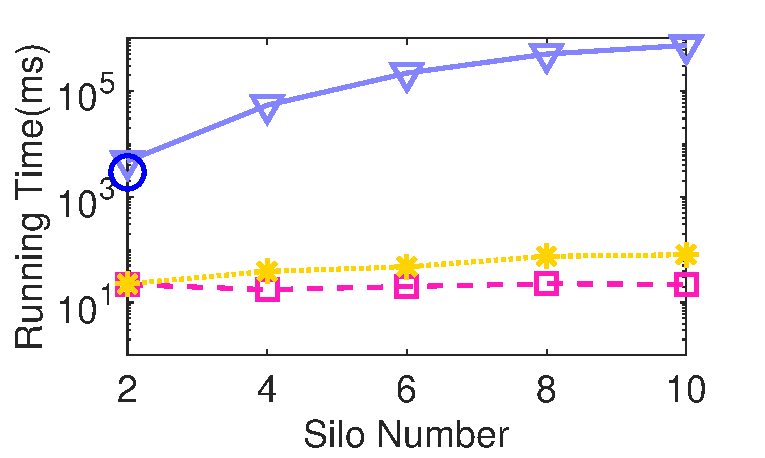
\includegraphics[width=0.48\linewidth]{apdx/knn_silo_time.pdf}
        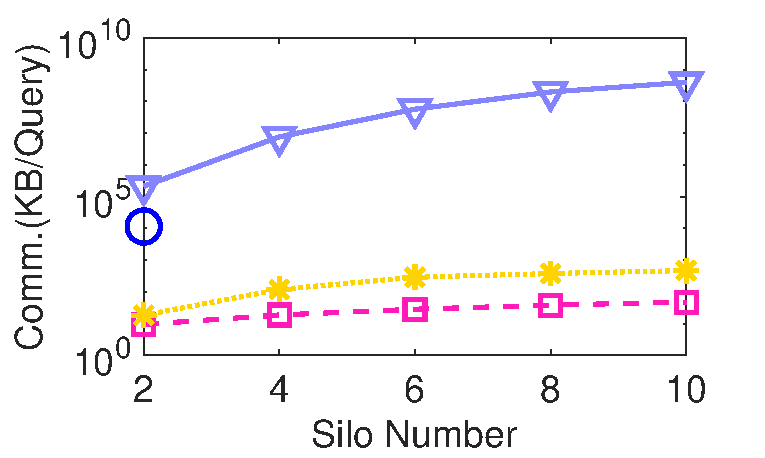
\includegraphics[width=0.48\linewidth]{apdx/knn_silo_cost.pdf}
        \caption{Running time and communication cost of (asymmetric) federated kNN query}
        \label{fig:knn-eff-silo-n-ho}
    \end{subfigure}
    \begin{subfigure}{0.48\textwidth}
        \centering
        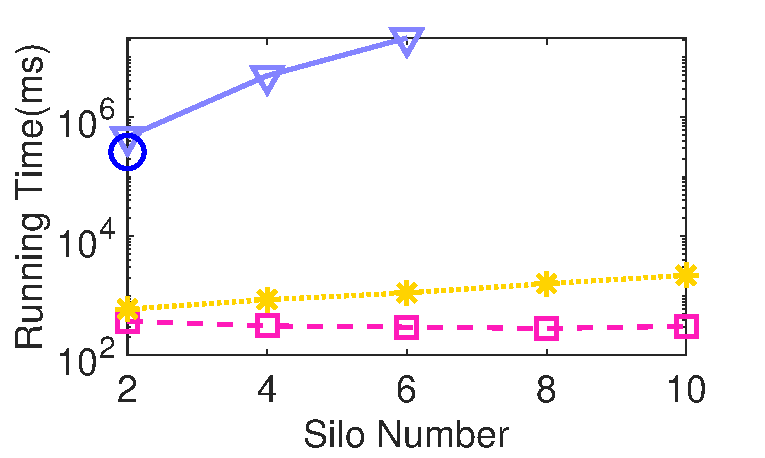
\includegraphics[width=0.48\linewidth]{apdx/knnjoin_silo_time.pdf}
        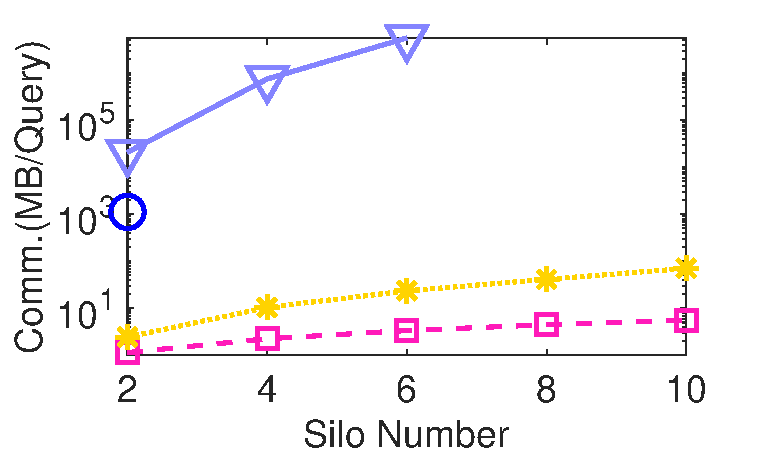
\includegraphics[width=0.48\linewidth]{apdx/knnjoin_silo_cost.pdf}
        \caption{Running time and communication cost of (asymmetric) federated kNN join}
        \label{fig:knn-j-eff-silo-n-ho}
    \end{subfigure}
    \begin{subfigure}{0.48\textwidth}
        \centering
        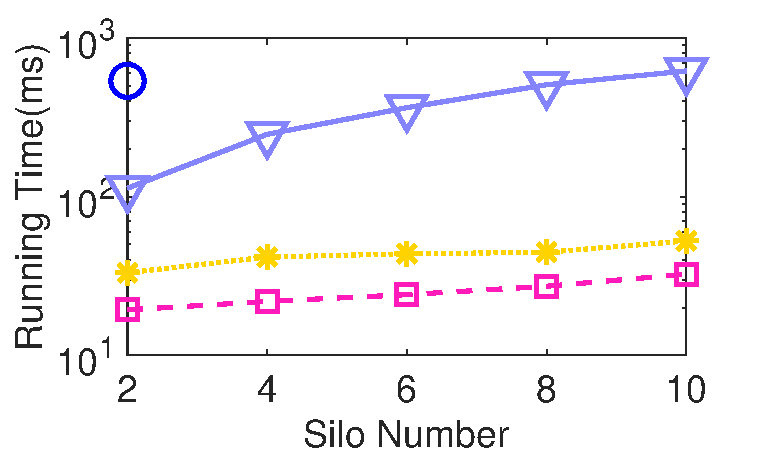
\includegraphics[width=0.48\linewidth]{apdx/rangecount_silo_time.pdf}
        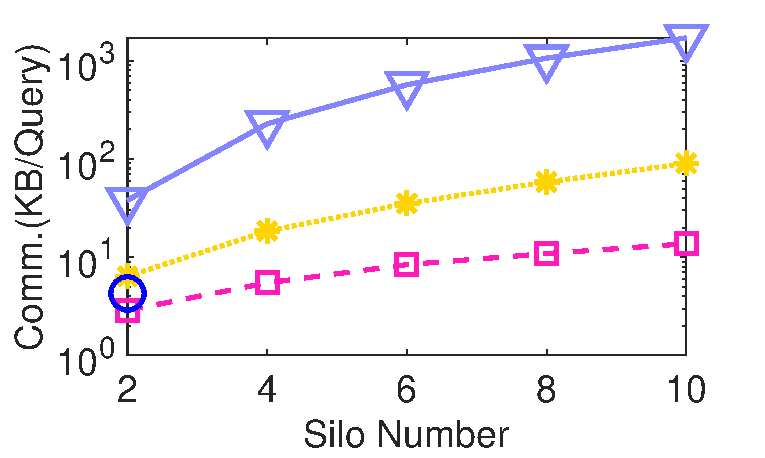
\includegraphics[width=0.48\linewidth]{apdx/rangecount_silo_cost.pdf}
        \caption{Running time and communication cost of (asymmetric) federated range counting}
        \label{fig:count-eff-silo-n-ho}
    \end{subfigure}
     \begin{subfigure}{0.48\textwidth}
        \centering
        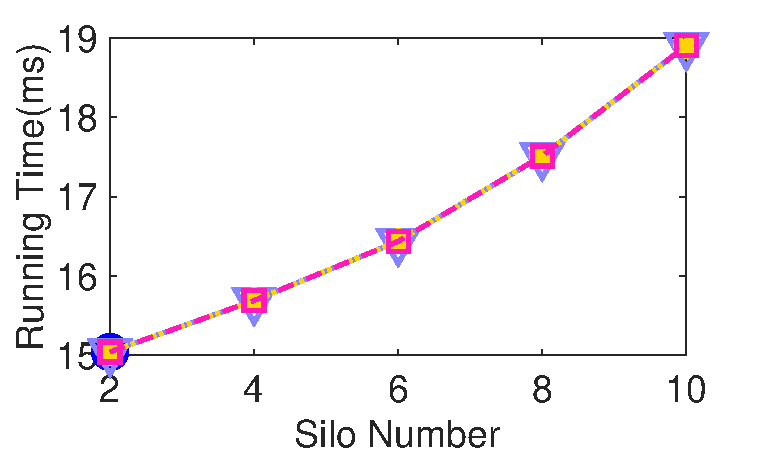
\includegraphics[width=0.48\linewidth]{apdx/rangequery_silo_time.pdf}
        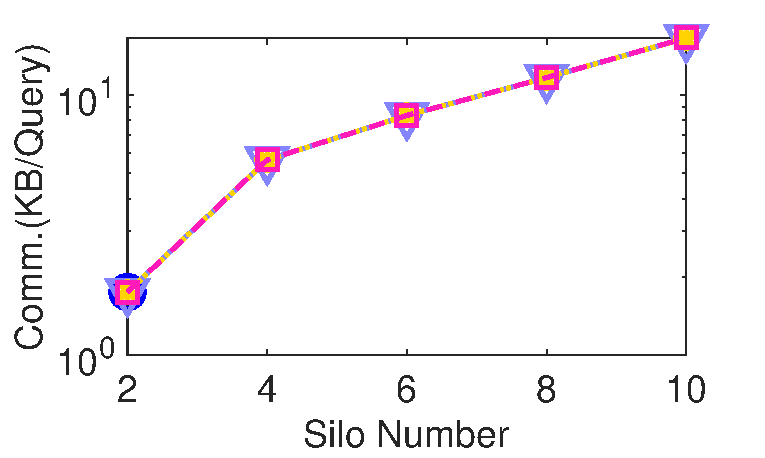
\includegraphics[width=0.48\linewidth]{apdx/rangequery_silo_cost.pdf}
        \caption{Running time and communication cost of (asymmetric) federated range query}
        \label{fig:range-eff-silo-n-ho}
    \end{subfigure}
    \begin{subfigure}{0.48\textwidth}
        \centering
        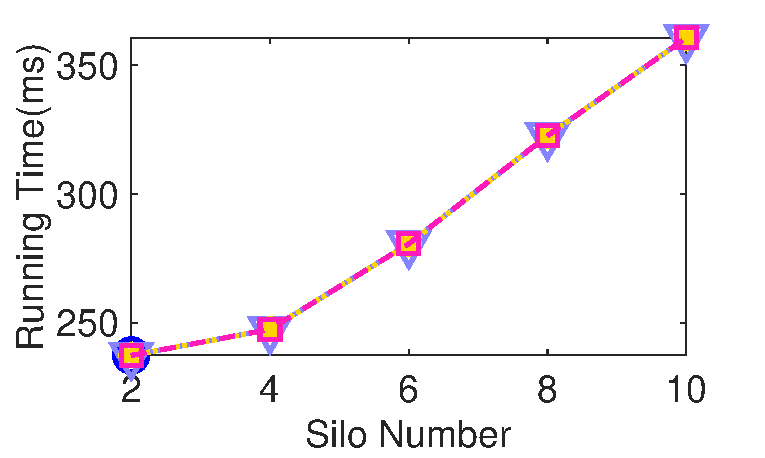
\includegraphics[width=0.48\linewidth]{apdx/dj_silo_time.pdf}
        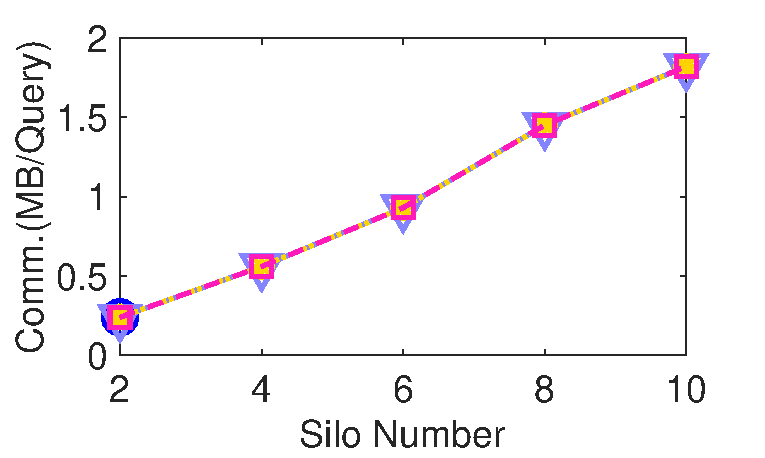
\includegraphics[width=0.48\linewidth]{apdx/dj_silo_cost.pdf}
        \caption{Running time and communication cost of (asymmetric) federated distance join}
    \end{subfigure}
    \caption{\sysname with an honest broker varying the silo number.}
    \label{fig:exp-honest-silo}
\end{figure}

\begin{figure}[t]
    \begin{subfigure}{0.45\textwidth}
        \centering
        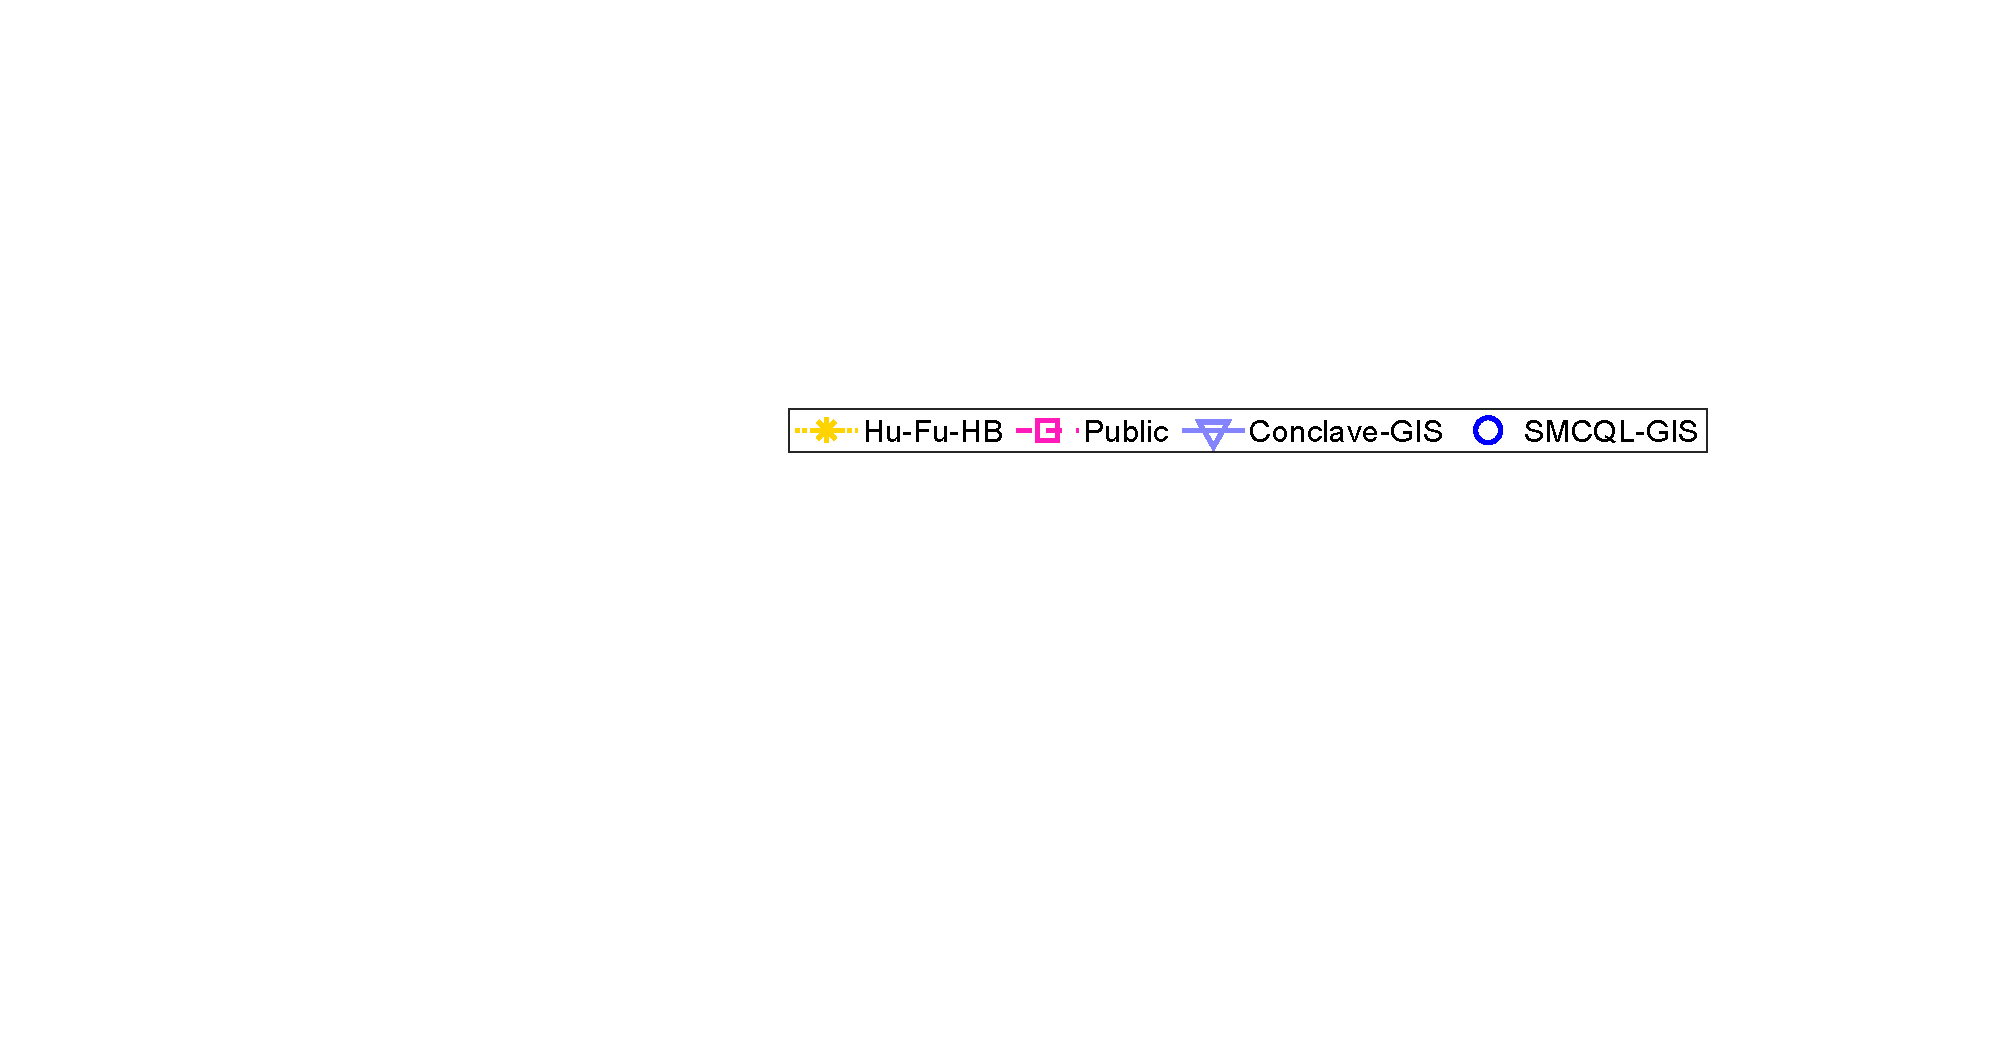
\includegraphics[width=\textwidth]{apdx/legend.pdf}
    \end{subfigure}
     \begin{subfigure}{0.48\textwidth}
        \centering
        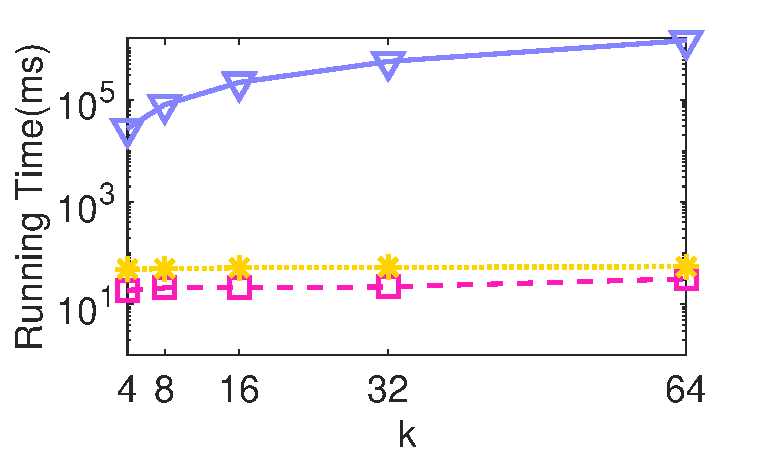
\includegraphics[width=0.48\linewidth]{apdx/knn_k_time.pdf}
        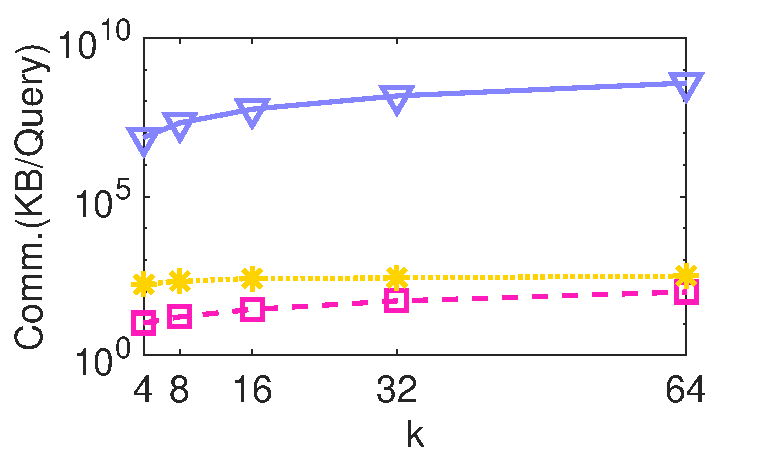
\includegraphics[width=0.48\linewidth]{apdx/knn_k_cost.pdf}
        \caption{Running time and communication cost of (asymmetric) federated kNN query}
        \label{fig:knn-eff-k-n-hon}
    \end{subfigure}  
     \begin{subfigure}{0.48\textwidth}
        \centering
        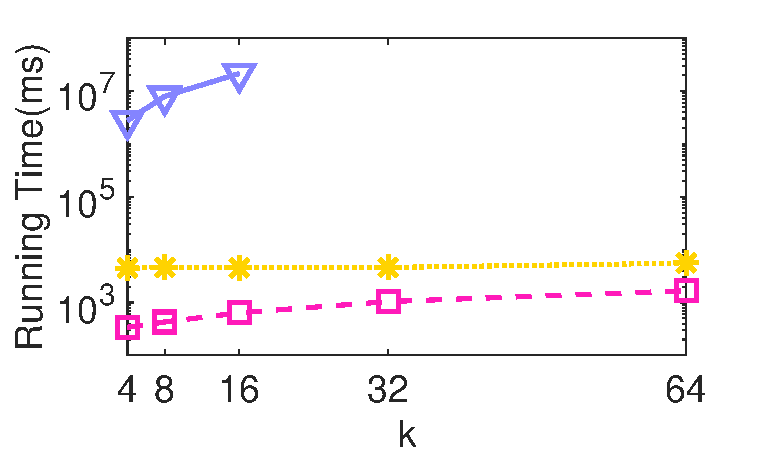
\includegraphics[width=0.48\linewidth]{apdx/knnjoin_k_time.pdf}
        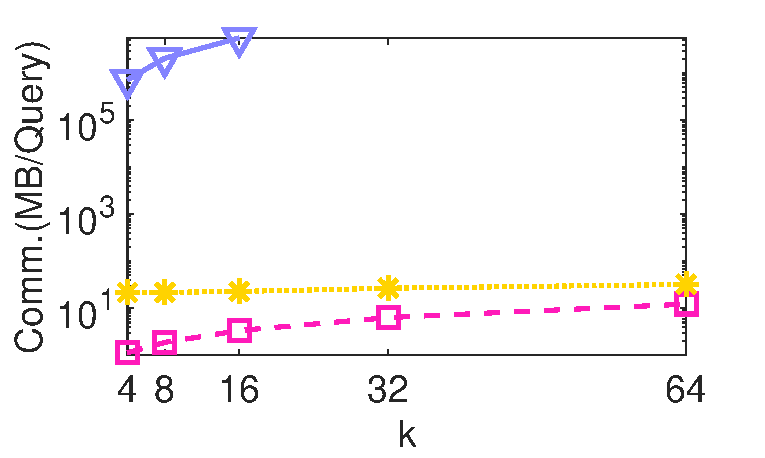
\includegraphics[width=0.48\linewidth]{apdx/knnjoin_k_cost.pdf}
        \caption{Running time and communication cost of (asymmetric) federated kNN join}
        \label{fig:knn-j-eff-k-n-hon}
    \end{subfigure} 
     \begin{subfigure}{0.48\textwidth}
        \centering
        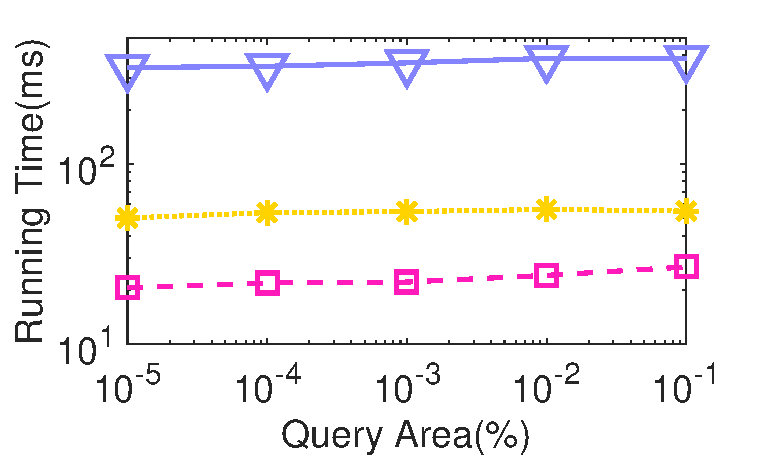
\includegraphics[width=0.48\linewidth]{apdx/rangecount_area_time.pdf}
        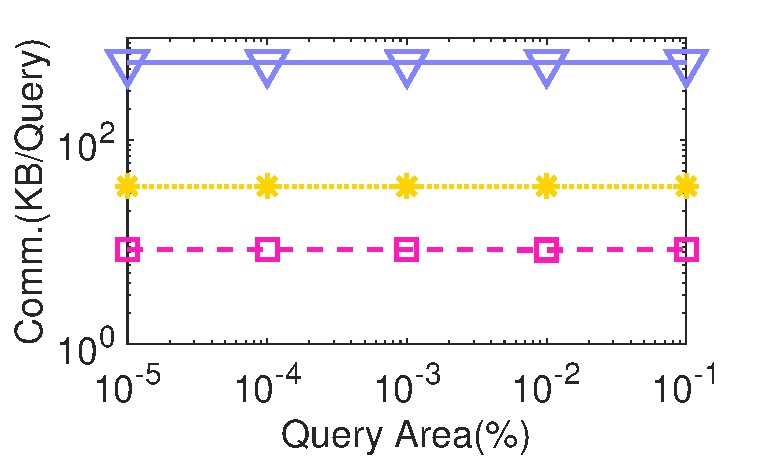
\includegraphics[width=0.48\linewidth]{apdx/rangecount_area_cost.pdf}
        \caption{Running time and communication cost of (asymmetric) federated range counting}
        \label{fig:count-eff-r-n-hon}
    \end{subfigure}
     \begin{subfigure}{0.48\textwidth}
        \centering
        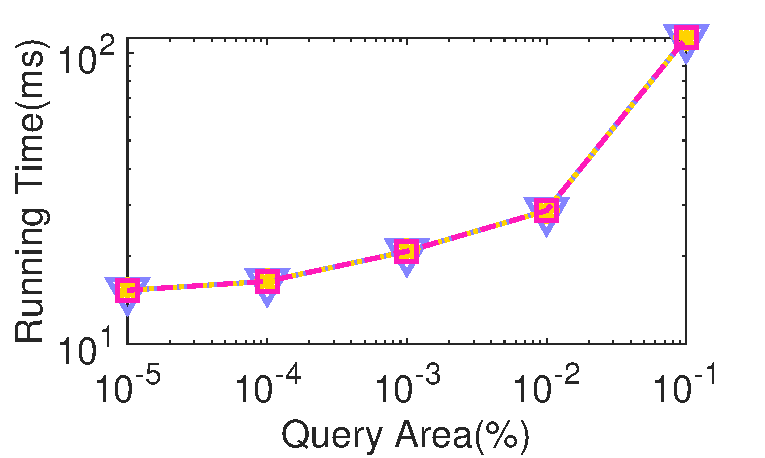
\includegraphics[width=0.48\linewidth]{apdx/rangequery_area_time.pdf}
        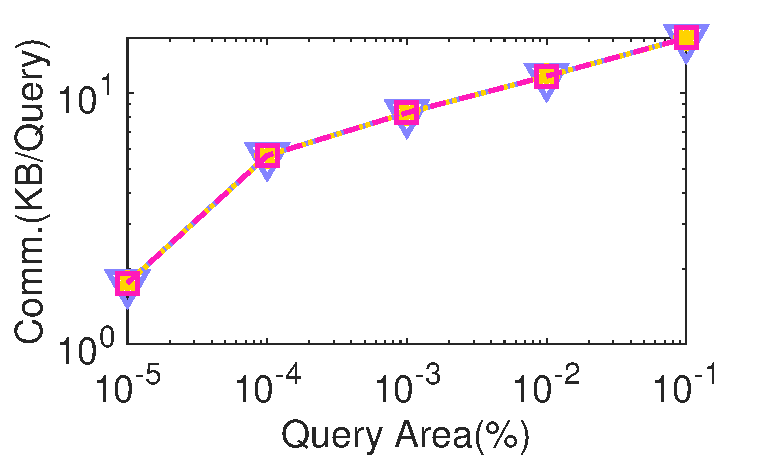
\includegraphics[width=0.48\linewidth]{apdx/rangequery_area_cost.pdf}
        \caption{Running time and communication cost of (asymmetric) federated range query}
        \label{fig:range-eff-r-n-hon}
    \end{subfigure}
      \begin{subfigure}{0.48\textwidth}
        \centering
        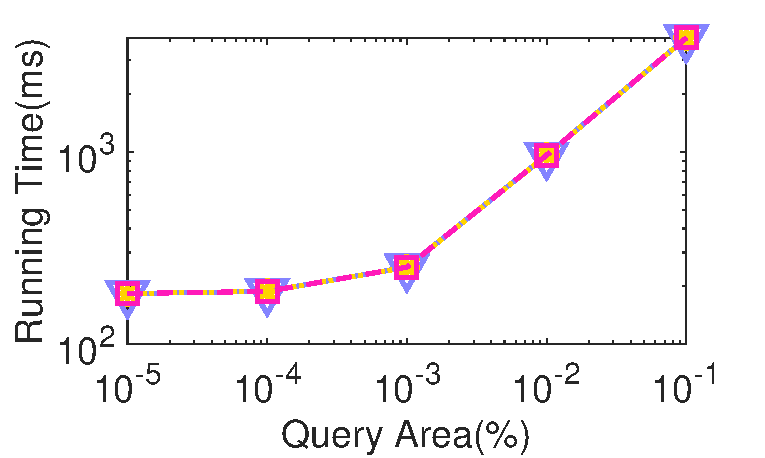
\includegraphics[width=0.48\linewidth]{apdx/dj_area_time.pdf}
        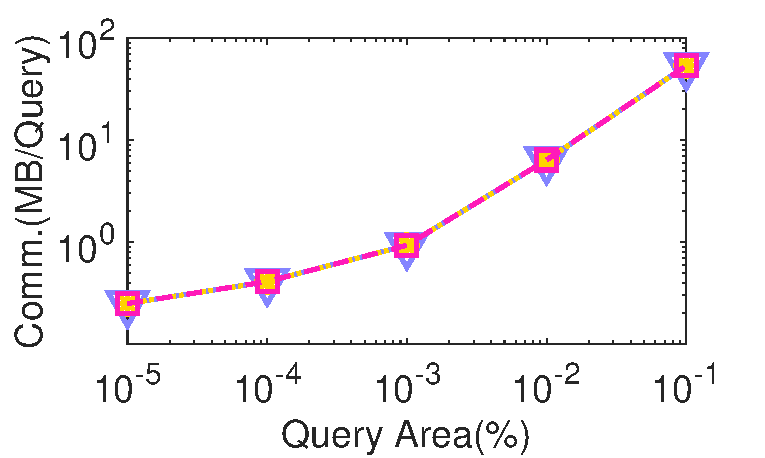
\includegraphics[width=0.48\linewidth]{apdx/dj_area_cost.pdf}
        \caption{Running time and communication cost of (asymmetric) federated distance join}
        \label{fig:dj-eff-r-n-hon}
    \end{subfigure}  
    \caption{\sysname with an honest broker varying the query-specific parameter.}
    \label{fig:exp-honest-para}
\end{figure}

\section{Experiment on \sysname with an Honest Broker} \label{app:exp-hb}
In the following, we conduct an experiment to demonstrate the performance of \sysname with an honest broker (denoted by ``\sysname-HB'').

\fakeparagraph{Experimental Setup}
This experiment has tested all asymmetric federated spatial queries on the real-world dataset BJ. We compare \sysname-HB with \smcql/\conclave in query processing efficiency measured in running time and communication overhead. Besides, the other experiment settings are the same as those in \secref{subsec:exp-cmp}.

\fakeparagraph{Experimental Result}
\figref{fig:exp-honest-silo} and \figref{fig:exp-honest-para} present the experimental results of \sysname-HB and \smcql/\conclave in terms of running time and communication cost. First, We can observe that \sysname-HB performs the same as \smcql and \conclave on asymmetric federated range query and distance join. This is because all the compared algorithms (including ours) are simplified to Public due to the honest broker who collects the partial results (\ie sensitive data) of plaintext range query in each silo and is assumed to never reveal them to anyone else. Second, as for federated range counting, kNN query and kNN join, \sysname-HB still outperforms \smcql and \conclave with up to 4 orders of magnitudes faster in running time and 5 orders of magnitudes lower in communication cost. This is because our query writer is more effective to process queries on large-scale spatial data.

\fakeparagraph{Summary}
The experimental results demonstrate that compared to \smcql and \conclave, \sysname-HB exhibits similar efficiency in performing asymmetric federated range queries and distance joins. Additionally, \sysname-HB achieves better efficiency in asymmetric federated range counting, kNN queries, and kNN joins.
Although this experiment primarily focuses on asymmetric federated spatial queries, the observed patterns also apply to symmetric federated spatial queries. 
Specifically, the efficiency of symmetric federated range queries, distance joins, kNN queries, and kNN joins can be improved when an honest broker is present and a secure set union can be avoided.
However, in contrast to these operations, symmetric federated range counting is not affected by the presence of an honest broker, as it does not involve a secure set union operator in its decomposition plan (as shown in \tabref{tab:sym-rewriter}).

\section{Experiment on Geographically Partitioned Dataset} \label{app:exp-geo}
To explore the performance of \sysname in the dataset where each silo corresponds to a single country, we have conducted an experiment on a new synthetic dataset (denoted by ``\textit{OSM country}'').

\begin{table}[t]
    \centering
    \caption{Percentage of data of each country in \textit{OSM country}.}
    \begin{tabular}{cc}
		\toprule
		Country & Percentage of data  \\
		\midrule
		China             & $21.7\%$        \\
		India             & $29.8\%$        \\
		Japan             & $39.4\%$        \\
		Malaysia          & $4.2\%$         \\
		North Korea       & $1.2\%$         \\
		South Korea       & $3.7\%$         \\
		\bottomrule
    \end{tabular}
    \label{tab:country}
\end{table}

\fakeparagraph{Experimental Setup}
The \textit{OSM country} dataset consists of spatial points from six countries in OpenStreetMap~\cite{osm}. These countries include China, India, Japan, Malaysia, North Korea and South Korea, and each of them corresponds to a single data silo. As shown in \tabref{tab:country}, the volume of data in each silo follows the native data proportion of the corresponding country in OpenStreetMap. For example, the numbers of data points in China, India and Japan are much larger than those of Malaysia, North Korea and South Korea. Here, we vary the total number of all data points from $10^4$ to $10^9$. 
The query workloads are mainly asymmetric federated spatial queries.
Besides, the other experiment parameters are the same as those in \secref{subsec:exp-asymm-scalability}.

\fakeparagraph{Experimental Result}
The results of this experiment are shown in \figref{fig:exp-cty}. First, we can observe that in the \textit{OSM country} dataset, \sysname also shows a significant improvement in both running time and communication cost over \conclave and \conclaveext on federated kNN query, kNN join and range counting. For example, \sysname is at least 3 orders of magnitude faster than \conclave and \conclaveext in federated kNN query and kNN join, and costs 5 orders of magnitude lower network communication. Second, \sysname achieves the same efficiency as \conclaveext on federated range query and distance join. Overall, the ranking of the compared solutions in terms of either running time or communication cost is consistent with the ranking in \secref{subsec:exp-scalability}. Note that we exclude \conclaveext from the results of federated range counting as shown in \figref{fig:count-eff-size-n-cty}, because this query does not need the secure set union to protect data ownership in this query.

\begin{figure}[t]
    \begin{subfigure}{0.45\textwidth}
        \centering
        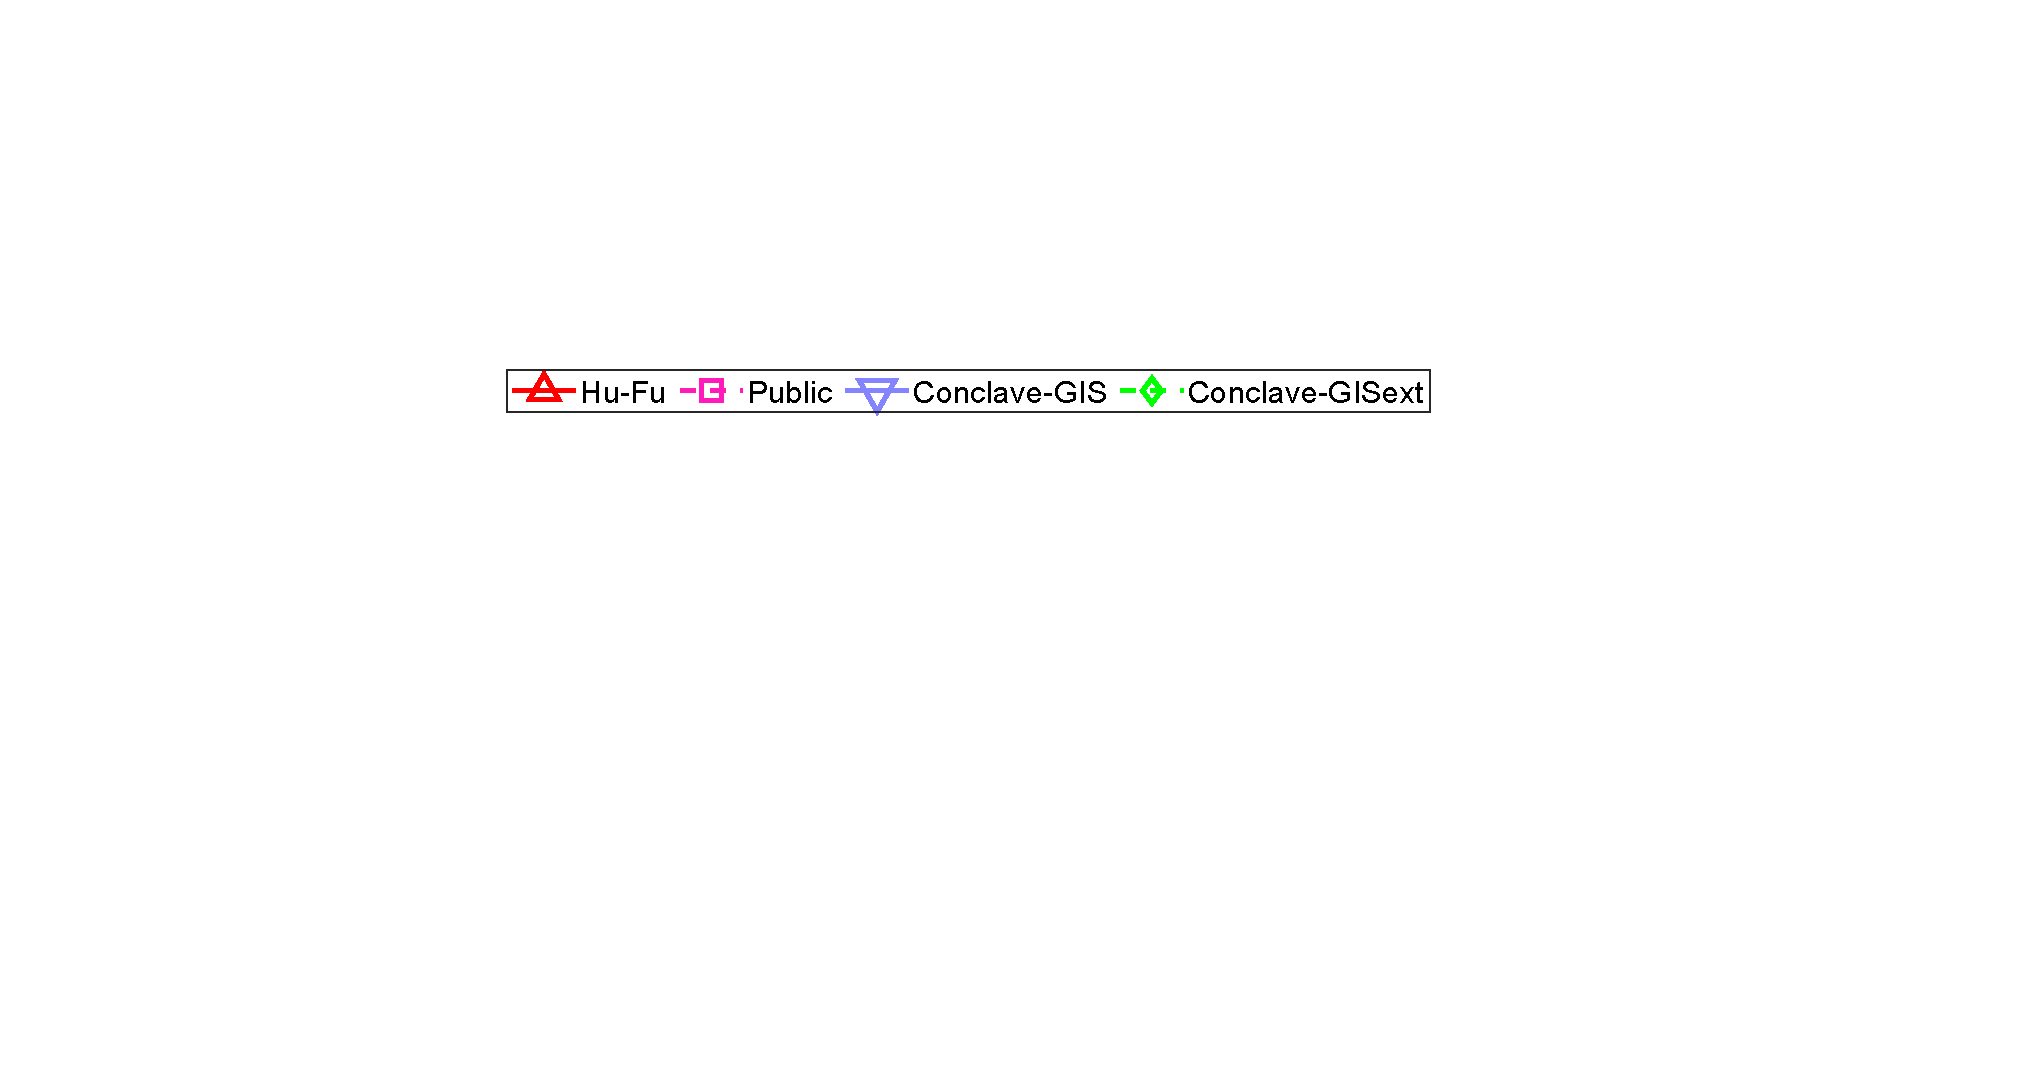
\includegraphics[width=\textwidth]{apdx/legend_scalability.pdf}
    \end{subfigure}
    \begin{subfigure}{0.48\textwidth}
        \centering
        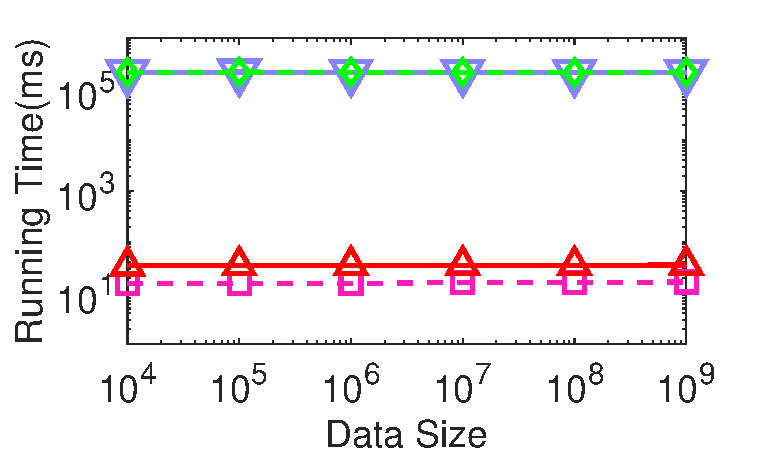
\includegraphics[width=0.48\linewidth]{apdx/knn_datasize_time_revision.pdf}
        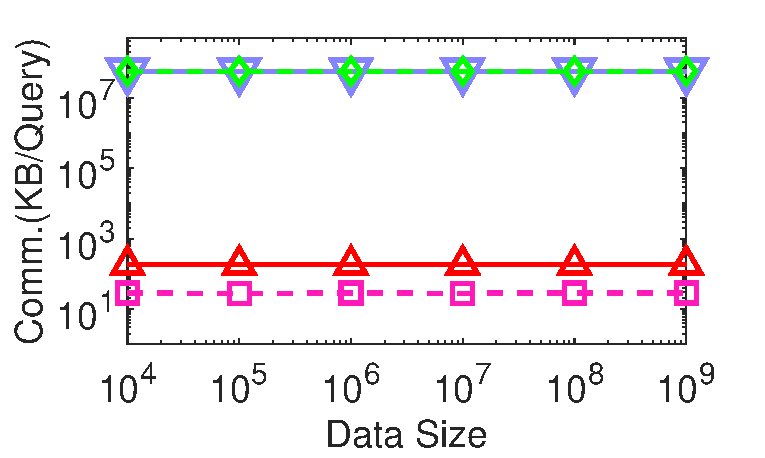
\includegraphics[width=0.48\linewidth]{apdx/knn_datasize_cost_revision.pdf}
        \caption{Running time and communication cost of (asymmetric) federated kNN query}
        \label{fig:knn-eff-size-n-cty}
    \end{subfigure}  
    \begin{subfigure}{0.48\textwidth}
        \centering
        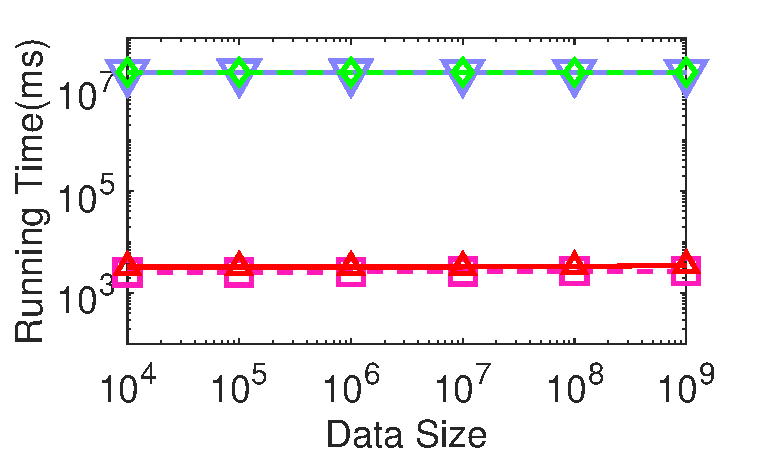
\includegraphics[width=0.48\linewidth]{apdx/knnjoin_datasize_time_revision.pdf}
        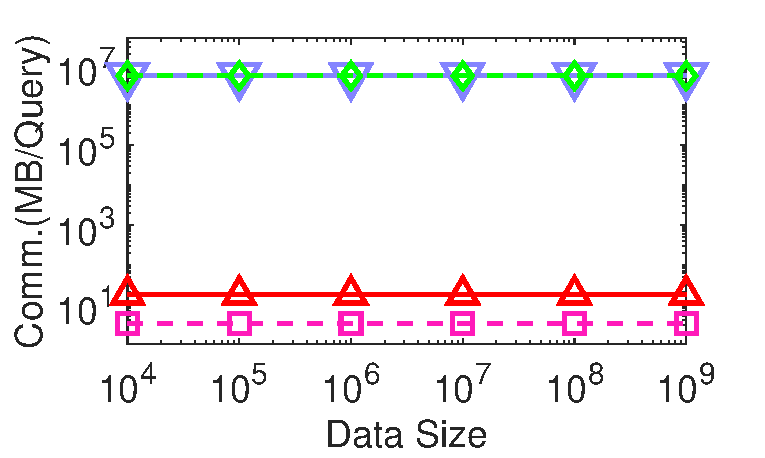
\includegraphics[width=0.48\linewidth]{apdx/knnjoin_datasize_cost_revision.pdf}
        \caption{Running time and communication cost of (asymmetric) federated kNN join}
        \label{fig:knn-j-eff-size-n-cty}
    \end{subfigure}  
    \begin{subfigure}{0.48\textwidth}
        \centering
        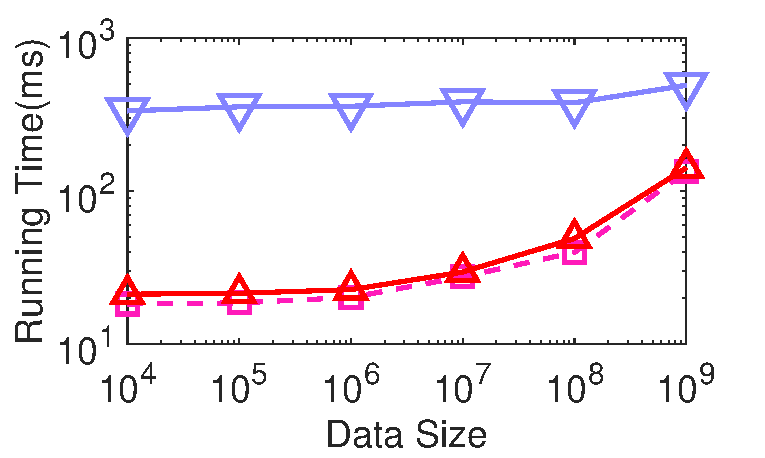
\includegraphics[width=0.48\linewidth]{apdx/rangecount_datasize_time_revision.pdf}
        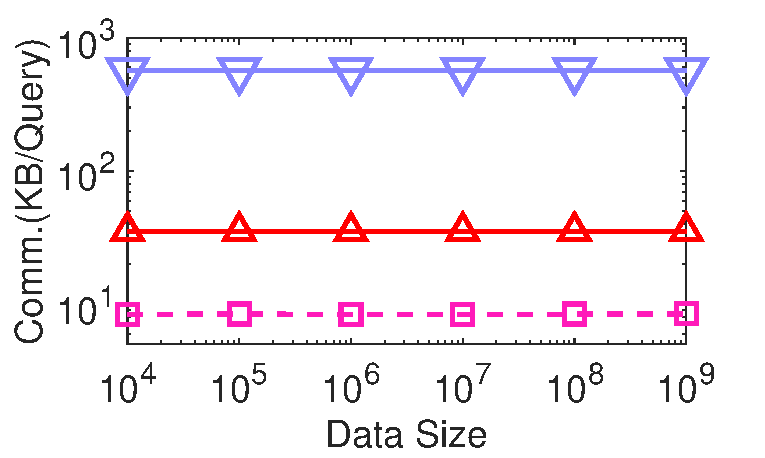
\includegraphics[width=0.48\linewidth]{apdx/rangecount_datasize_cost_revision.pdf}
        \caption{Running time and communication cost of (asymmetric) federated range counting}
        \label{fig:count-eff-size-n-cty}
    \end{subfigure}      
     \begin{subfigure}{0.48\textwidth}
        \centering
        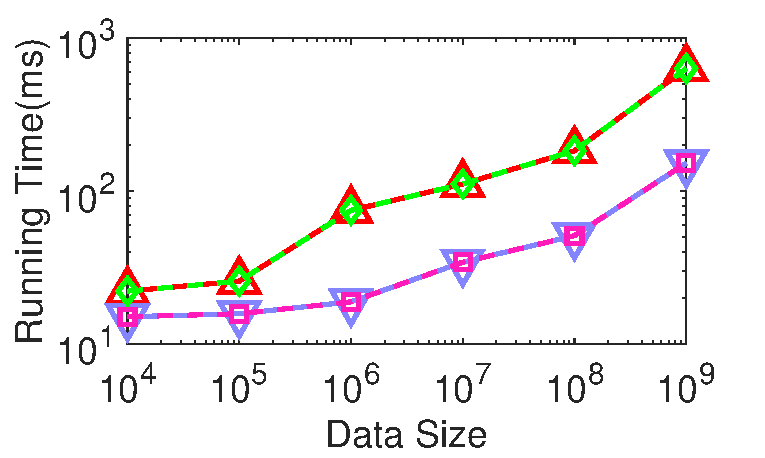
\includegraphics[width=0.48\linewidth]{apdx/rangequery_datasize_time_revision.pdf}
        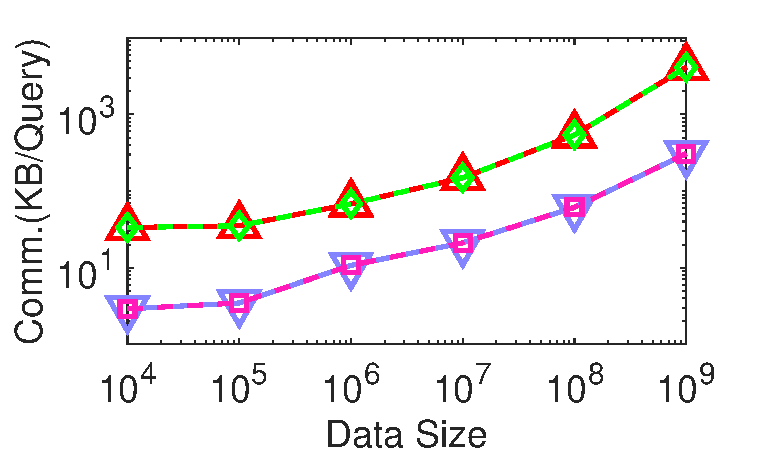
\includegraphics[width=0.48\linewidth]{apdx/rangequery_datasize_cost_revision.pdf}
        \caption{Running time and communication cost of (asymmetric) federated range query}
        \label{fig:range-eff-size-n-cty}
    \end{subfigure}      
     \begin{subfigure}{0.48\textwidth}
        \centering
        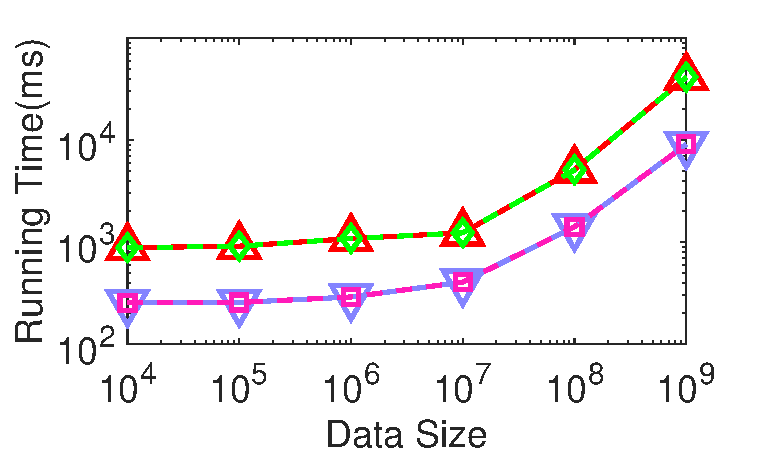
\includegraphics[width=0.48\linewidth]{apdx/dj_datasize_time_revision.pdf}
        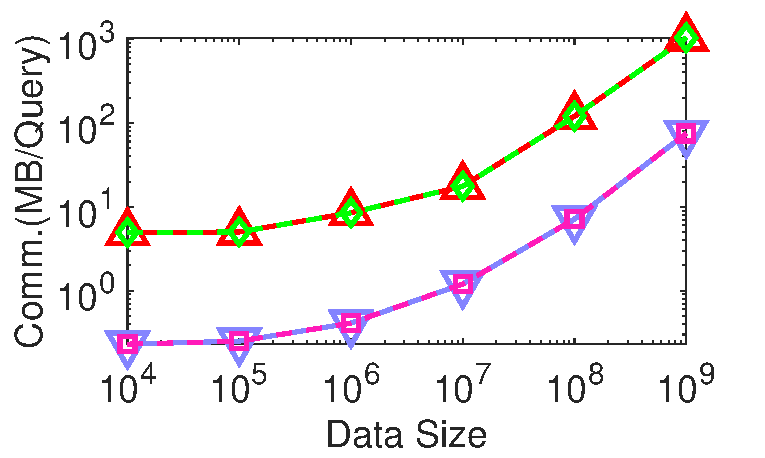
\includegraphics[width=0.48\linewidth]{apdx/dj_datasize_cost_revision.pdf}
        \caption{Running time and communication cost of (asymmetric) federated distance join}
    \end{subfigure}   
    \caption{Scalability test on synthetic dataset partitioned by countries.}
    \label{fig:exp-cty}
\end{figure}

\fakeparagraph{Summary}
In this evaluation, \sysname outperforms \smcqlext and \conclaveext in terms of efficiency for asymmetric federated kNN queries, kNN join, and range counting. 
Meanwhile, \sysname performs comparably to \smcqlext and \conclaveext for asymmetric federated range queries and distance join.
Thus, we can conclude that the experiment conducted on the \textit{OSM country} dataset yields similar results to those observed in \secref{subsec:exp-asymm-scalability}. This similarity may stem from the fact that none of the existing methods have leveraged the data distribution in their query processing strategies.
Similarly, this new data partition is unlikely to alter the overall performance ranking of symmetric federated spatial queries. 

\section{Experiment on the Improvement by the Index in Each Data Silo}
\label{appendix:spatial-index}
To demonstrate that the federated spatial queries have already been accelerated by local indexes in \sysname, we have conducted a new experiment on the efficiency improvement caused by these local indexes (\ie R-trees in our default setting).

\fakeparagraph{Experimental Setup}
In this experiment, we test the running time of the plaintext spatial queries in \sysname (\ie plaintext range query, plaintext range counting and plaintext kNN query) on PostgreSQL with and without an R-tree. And the plaintext spatial queries are processed on the OSM dataset. Besides, we vary the data size from $10^4$ to $10^8$ and use the default setting of query area (0.001\%) and $k$ (16). The other experiment settings are the same as those in \secref{sec:experiment-setup}.

\fakeparagraph{Experimental Result}
As shown in \figref{fig:plaintext_query_index}, local indexes can improve the efficiency of plaintext spatial queries, especially when the data size is large. Specifically, the local index (R-tree) reduces the running time by up to $40\times$, $44\times$ and $2042\times$ when processing plaintext range query, range counting, and kNN query, respectively. Moreover, the plaintext spatial queries without local indexes cost even longer time than corresponding federated spatial queries in \sysname. For instance, the running time of processing one federated kNN query by \sysname takes 52 ms when the data size is $10^8$, which is even faster than that of the plaintext kNN query without the local index (2465 ms). Thus, the experimental result proves that we have used local indexes in \sysname to speed up the processing of the plaintext operators.

\begin{figure}[t]
    \centering
    \begin{subfigure}{0.48\textwidth}
        \centering
        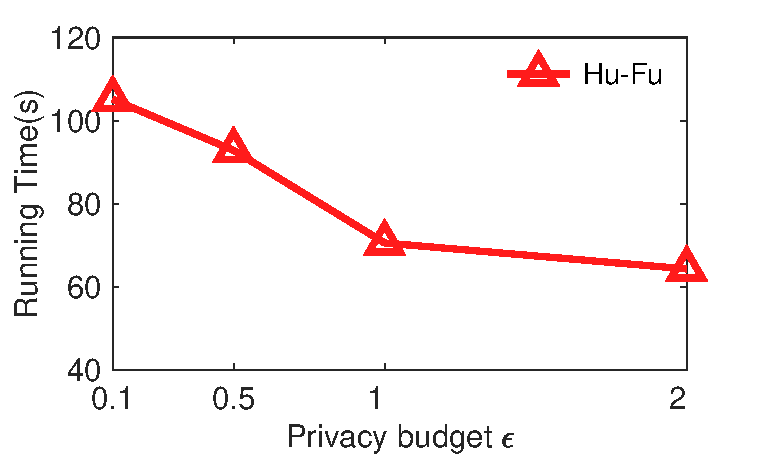
\includegraphics[width=0.48\linewidth]{apdx/epsilon_knnquery_time.pdf}
        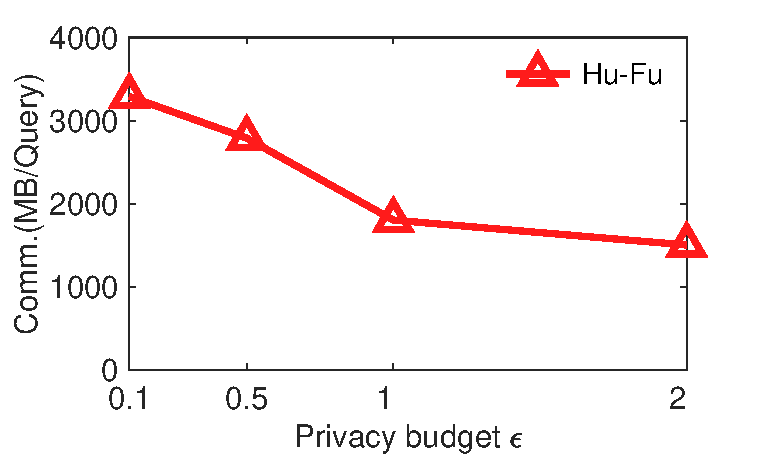
\includegraphics[width=0.48\linewidth]{apdx/epsilon_knnquery_comm.pdf}
        \caption{Runtime and communication cost of varying  $\epsilon$ in \sysname for processing symmetric federated kNN query}
        \label{fig:epsilon_knn}
    \end{subfigure}
    \begin{subfigure}{0.48\textwidth}
        \centering
        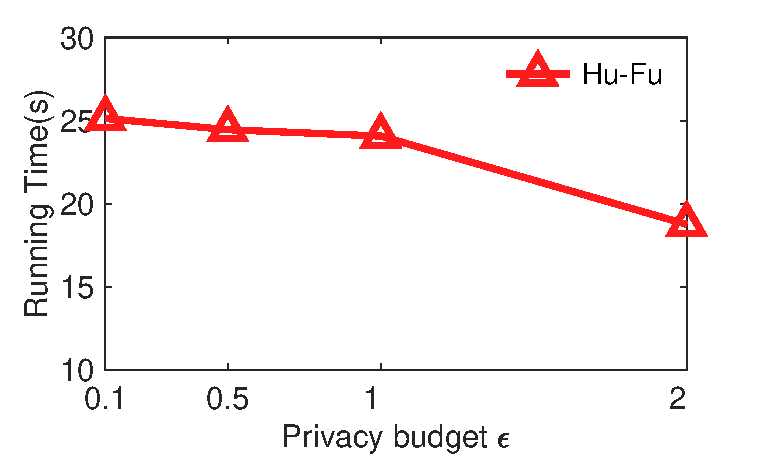
\includegraphics[width=0.48\linewidth]{apdx/epsilon_rangequery_time.pdf}
        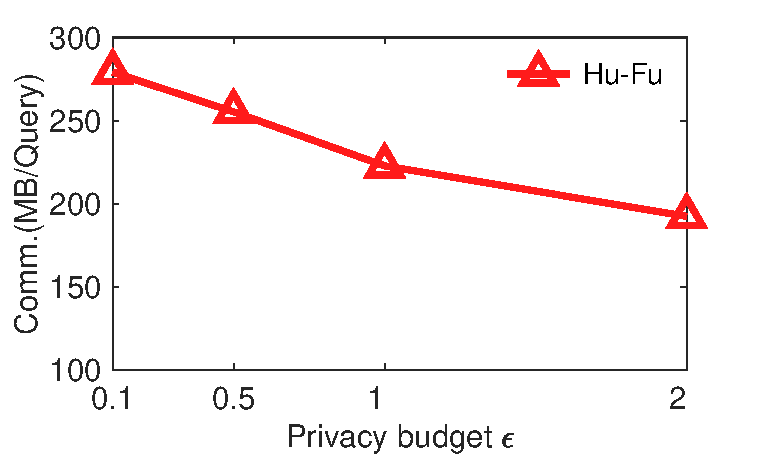
\includegraphics[width=0.48\linewidth]{apdx/epsilon_rangequery_comm.pdf}
        \caption{Runtime and communication cost of varying $\epsilon$ in \sysname for processing symmetric federated range query}
        \label{fig:epsilon_rangequery}
    \end{subfigure}
    \caption{Impact of privacy budget $\epsilon$ in \sysname for processing symmetric federated kNN and range queries.}
    \label{fig:epsilon_eff}
\end{figure}

\begin{figure*}[t]
    \centering
    \begin{subfigure}{0.32\textwidth}
        \centering
        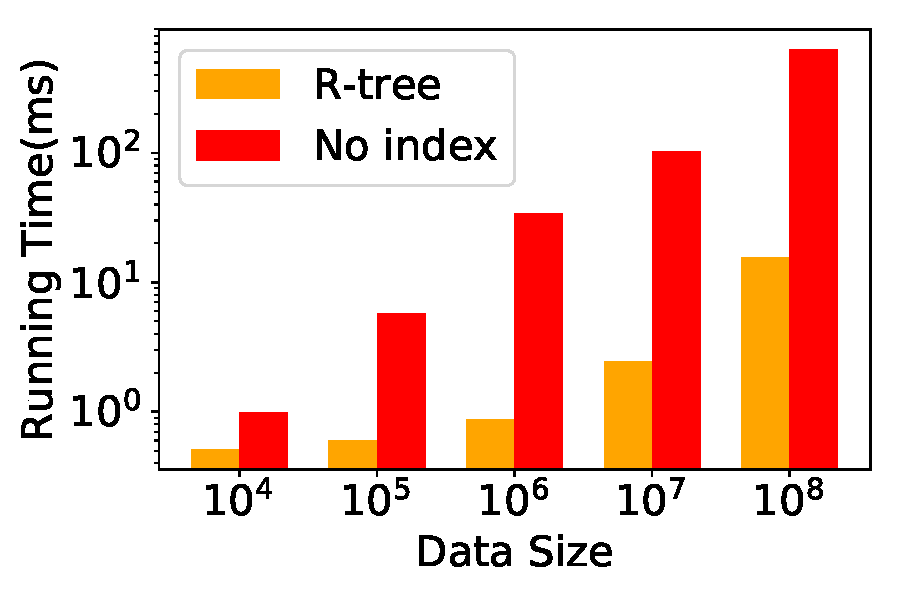
\includegraphics[width=\textwidth]{apdx/range_query_index.pdf}
        \caption{Plaintext range query}
        \label{fig:plain-range-query}
    \end{subfigure}
    ~
    \begin{subfigure}{0.32\textwidth}
        \centering
        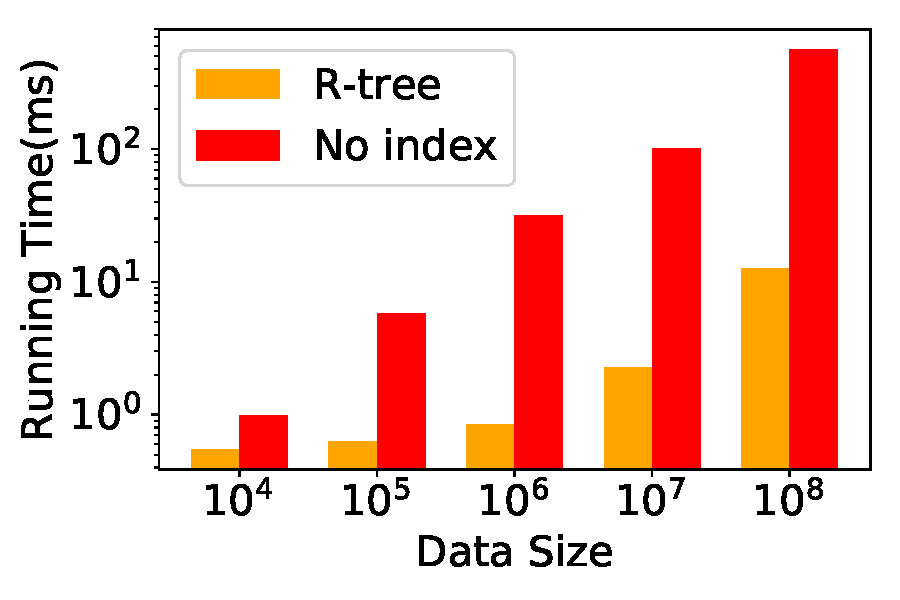
\includegraphics[width=\textwidth]{apdx/range_count_index.pdf}
        \caption{Plaintext range counting}
        \label{fig:plain-range-counting}
    \end{subfigure}
    ~
    \begin{subfigure}{0.32\textwidth}
        \centering
        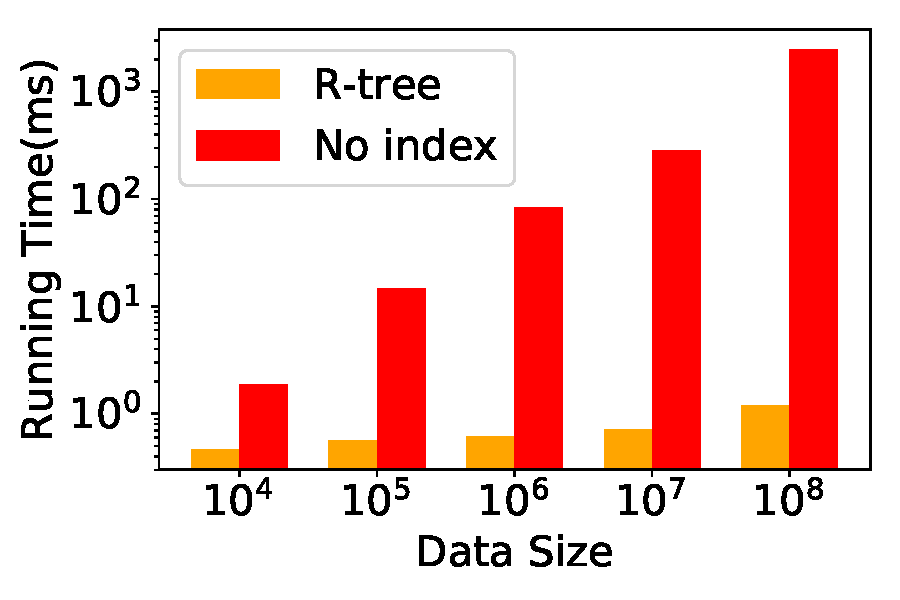
\includegraphics[width=\textwidth]{apdx/knn_index.pdf}
        \caption{Plaintext kNN query}
        \label{fig:plain-knn-query}
    \end{subfigure}
    ~
	\caption{Running time of plaintext spatial queries with/without R-tree.}
	\label{fig:plaintext_query_index}
\end{figure*}

\section{Impact of Additionally Protecting Query Privacy in Symmetric Queries on Time Cost}
\label{app:impact-query-privacy}

Symmetric queries generally exhibit slower performance compared to asymmetric queries.
The gap stems from the essential difference in the problem definition (\ie whether query privacy needs to be protected or not).
Consequently, accurately assessing the impact on time cost when incorporating query privacy protection is difficult.

However, we can roughly estimate the impact on time cost in two ways: 
\begin{itemize}
    \item By comparing the number of basic operators required for symmetric queries and asymmetric queries in \tabref{tab:sym-rewriter} and \tabref{tab:rewriter}, we can conclude that symmetric queries incur higher costs than asymmetric queries.
    For example, a symmetric federated range query involves many more secure operators (\eg secure distance comparisons) than an asymmetric federated range query.
    This explains why the former generally exhibits slower performance than the latter.
    
    \item We also report the impact on time cost under the default experimental setting.
    To obtain the result, we evaluate both \sysname and \conclave for asymmetric federated range query and range counting on real-world dataset BJ in our new experimental environment.
    As shown in \tabref{tab:asym-slow-sym}, a symmetric federated range query using \conclave is 4,054$\times$ slower than the corresponding asymmetric query.
    By contrast, our solution \sysname significantly narrows this gap to 59$\times$.
    We can observe a similar pattern for federated range counting.
    Although there is still a notable difference in the time cost between symmetric queries and asymmetric queries by using \sysname, \tabref{tab:asym-slow-sym} demonstrates that \sysname performs better in terms of query efficiency than the existing baseline, highlighting the challenge of achieving good efficiency for symmetric queries compared to asymmetric queries.
\end{itemize}

\begin{table*}[t]  
\centering
\caption{How many times slower is a symmetric query compared to an asymmetric query by specific solution}\label{tab:asym-slow-sym}
\begin{tabular}{ccc}  
\toprule   
Solution			 & Federated Range Query & Federated Range Counting \\ \midrule
\conclave & 4054$\times$ & 5302$\times$ \\ 
\sysname & 59$\times$ & 77$\times$ \\  
\bottomrule
\end{tabular}  
\end{table*}

\section{Impact of Privacy Budget $\epsilon$ in Symmetric Queries}
\label{app:budget}
We use symmetric federated kNN and range queries to evaluate the impact of privacy budget $\epsilon$ on the query efficiency.
The impact of $\epsilon$ for symmetric federated range counting and distance join is similar to that for symmetric federated range query, 
and the impact of $\epsilon$ for symmetric federated kNN join is similar to that of symmetric federated kNN query.

Specifically, we use the real-world dataset BJ to conduct the evaluation, and vary the privacy budget $\epsilon$ within a range from 0.1 to 2, where $\epsilon=0.1$ indicates tighter privacy preservation level than $\epsilon=2$.
As for the other parameter settings, we use the default setting as introduced in Section 7.2.

\figref{fig:epsilon_eff} illustrates the running time and communication cost associated with symmetric federated kNN and range queries. As $\epsilon$ increases from 0.1 to 2, we observe a modest drop in both running time and communication cost for symmetric federated kNN query. 
A similar trend  is also evident in the results of the symmetric federated range query. The overall pattern is reasonable, since a larger $\epsilon$ indicates a more relaxed privacy protection requirement, which results in a shorter distance between the query object and its perturbed location.